%% Classe du document
\documentclass[a4paper,10pt]{article}

%% Francisation
\usepackage[francais]{babel} % Indique que l'on utilise le francais
\usepackage[T1]{fontenc}
\usepackage[utf8]{inputenc} % Indique que l'on utilise tout le clavier
%\usepackage[latin1]{inputenc}

%% Réglages généraux
\usepackage[top=3cm, bottom=3cm, left=3cm, right=3cm]{geometry} % Taille de la feuille
\usepackage{lastpage}

%% Package pour le texte
\usepackage{soul} % Souligner
\usepackage{color} % Utilisation de couleurs
\usepackage{hyperref} % Créer des liens et des signets
\usepackage{eurosym}% Pour le symbole euro
\usepackage{fancyhdr}% Entête et pied de page

%% Package pour les tableaux
\usepackage{multirow} % Colonnes multiples
\usepackage{cellspace}
\usepackage{array}

%% Package pour les dessins
\usepackage{pstricks}
\usepackage{graphicx} % Importer des images
\usepackage{pdftricks} % Pour utiliser avec pdfTex
\usepackage{pst-pdf} % Pour utiliser avec pdfTex
\usepackage{pst-node} % Pose de noeuds
\usepackage{subfig}
\usepackage{float}

%% Package pour les maths
\usepackage{amsmath} % Commandes essentielles
\usepackage{amssymb} % Principaux symboles

%% Package pour le code
\usepackage{listings} % Utilisation de la couleur syntaxique des langages
\usepackage{url}


\usepackage[babel=true]{csquotes} % Permet les quotations (guillemets)
\usepackage{tocvsec2}
\usepackage{amsthm}
\usepackage{amsfonts}

\usepackage{tikz}
\usepackage{pdfpages}

\usetikzlibrary{shapes} % A revoir

%--------------------- Autres définitions ---------------------%

% Propriété des liens
\hypersetup{
colorlinks = true, % Colorise les liens
urlcolor = blue, % Couleur des hyperliens
linkcolor = black, % Couleur des liens internes
}

\definecolor{grey}{rgb}{0.95,0.95,0.95}

% Language Definitions for Turtle
%TODO: a revoir avec les couleur de gedit
\definecolor{olivegreen}{rgb}{0.2,0.8,0.5}
\definecolor{grey2}{rgb}{0.5,0.5,0.5}
\lstdefinelanguage{ttl}{
sensitive=true,
morecomment=[s][\color{grey2}]{@}{:},
morecomment=[l][\color{olivegreen}]{\#},
morecomment=[s][\color{red}]{<}{/>},
morestring=[s][\color{olivegreen}]{<http://w}{\#>},
morestring=[b][\color{blue}]{\"},
}

\lstset{
frame=single,
breaklines=true,
basicstyle=\ttfamily,
backgroundcolor=\color{grey},
basicstyle=\scriptsize,
keywordstyle=\color{blue},
commentstyle=\color{green},
stringstyle=\color{red},
identifierstyle=\color{blue}
}

%Definition de la commande pour retirer l'espace devant les ':'
\makeatletter
\@ifpackageloaded{babel}%
        {\newcommand{\nospace}[1]{{\NoAutoSpaceBeforeFDP{}#1}}}%  % !! double {{}} pour cantonner l'effet à l'argument #1 !!
        {\newcommand{\nospace}[1]{#1}}
\makeatother

\setcounter{tocdepth}{3}
%\maxsecnumdepth{subsubsection} % Dernière section numérotée

\newcommand{\paperPrototyping}{\emph{paper prototyping}}

% Corps du document :
\begin{document}

% Définition des entêtes et pieds de page
\fancyhead[LE,CE,RE,LO,CO,RO]{}
\fancyfoot[LE,CE,RE,LO,CO,RO]{}
\fancyhead[LO, LE]{Interface Homme-Machine 1}
\fancyhead[RO,RE]{2012/2013}
\fancyfoot[LO,LE]{Université de \scshape{Nantes}}
\fancyfoot[RO,RE]{Page \thepage \ sur \pageref{LastPage}}
\renewcommand{\headrulewidth}{0.4pt}
\renewcommand{\footrulewidth}{0.4pt}

%\maketitle
\begin{titlepage}

\vspace*{\fill}~
\begin{center}
{\large \textsc{Rapport de Projet}} \\
\vspace{1cm}
{\LARGE Projet : Gestionnaire de listes de tâches} \\
\vspace{1cm}
\textbf{Taskinator} \\

\includegraphics[height=1cm]{Images/Taskinator.png} \\
\vspace{1cm}
COUTABLE Guillaume, RULLIER Noémie \\
\today
\end{center}
\vspace*{\fill}

\vspace{\stretch{1}}
\begin{center}
\noindent 

\includegraphics[height=2.5cm]{Images/universite.png}
\end{center}
\pagebreak
\end{titlepage}

\newpage
\tableofcontents  

% Introduction
\newpage
\pagestyle{fancy}

%%%%%%%%%%%%%%%%%%%%%%%%%%%%%%%%%%%%%%%%%%%%%%%%%%%%%%%%%%%%%%%%%%%%%%%%%%%%%
%%%%%%%%%%  Introduction générale
%%%%%%%%%%%%%%%%%%%%%%%%%%%%%%%%%%%%%%%%%%%%%%%%%%%%%%%%%%%%%%%%%%%%%%%%%%%%%
\section{Introduction}
L'objectif de ce projet fut de développer un gestionnaire avancé de tâches. Celui-ci devait permettre de créer des listes de tâches et de suivre l'avancement
de celles-ci.

Afin de créer cette application que nous avons appelé \textit{Taskinator}, nous avons établit plusieurs étapes dans l'avancement du projet. Ce rapport
présentera  ces étapes  les unes après  les autres.

%%%%%%%%%%%%%%%%%%%%%%%%%%%%%%%%%%%%%%%%%%%%%%%%%%%%%%%%%%%%%%%%%%%%%%%%%%%%%
%%%%%%%%%%  Etape 1
%%%%%%%%%%%%%%%%%%%%%%%%%%%%%%%%%%%%%%%%%%%%%%%%%%%%%%%%%%%%%%%%%%%%%%%%%%%%%
\newpage
\section{Les fonctionnalités}
La première étape fut d'analyser l'ensemble des fonctionnalités que notre application devait proposer. 

\subsection{Fonctionnalités principales}
Voici dans un premier temps les fonctionnalités principales:
\paragraph{Créer une liste:} cette fonctionnalité permet à l'utilisateur de créer une liste non ordonnée vide.
\paragraph{Créer une liste ordonnée:} cette fonctionnalité permet à l'utilisateur de créer une liste ordonnée vide. L'ensemble des éléments de cette liste
doivent être effectués dans un ordre précis.
\paragraph{Créer une tâche:} cette fonctionnalité permet à l'utilisateur de créer une tâche.
\paragraph{Supprimer un élément:} cette fonctionnalité permet de supprimer une tâche ou une liste (ordonnée ou non). Cette fonctionnalité est à manipuler avec
précaution, en effet dans le cas d'une liste, la suppression de celle-ci implique aussi la suppression de tous ses éléments (listes ou tâches).
\paragraph{Enregistrer:} cette fonctionnalité permet à l'utilisateur d'enregistrer sa liste dans un fichier sur son disque dur.
\paragraph{Enregistrer un template:} cette fonctionnalité permet à l'utilisateur d'enregistrer la liste qu'il vient de créer comme un template afin que la
structure de celle-ci soit réutilisable.
\paragraph{Ouvrir un template:} cette fonctionnalité permet à l'utilisateur de créer une liste à partir d'un template enregistré. Il devra cependant renseigner
le nom de cette liste ainsi que toutes les dates de tous les éléments. Il peut ensuite continuer à modifier cette liste.

\subsection{Fonctionnalités secondaires}
Voici les fonctionnalités secondaires:
\paragraph{Paramètre:} cette fonctionnalité permet à l'utilisateur de modifier le type de l'élément sélectionné. Il pourra par exemple choisir de modifier une
liste en liste ordonnée ou en une tâche. Cette fonctionnalité est à manipuler avec précaution, en effet si l'utilisateur décide de transformer une liste en
tâche l'ensemble des éléments de la liste seront supprimés.
\paragraph{Monter / Descendre:} cette fonctionnalité permet de monter ou descendre un élément dans l'arborescence de la liste. Dans le cas d'une liste, tous
ces éléments sont aussi montés/descendus d'un rang. Si le changement se fait au sein d'une liste ordonnée l'ordre des éléments est aussi changé.
\paragraph{Aperçu:} cette fonctionnalité permet à l'utilisateur d'avoir un aperçu de sa liste, se qui permettra l'affichage d'un nombre plus important de
tâches.
\paragraph{Gérer ses templates:} cette fonctionnalité permet à l'utilisateur d'ajouter et de supprimer des templates.

%%%%%%%%%%%%%%%%%%%%%%%%%%%%%%%%%%%%%%%%%%%%%%%%%%%%%%%%%%%%%%%%%%%%%%%%%%%%%
%%%%%%%%%%  Etape 2
%%%%%%%%%%%%%%%%%%%%%%%%%%%%%%%%%%%%%%%%%%%%%%%%%%%%%%%%%%%%%%%%%%%%%%%%%%%%%
\newpage
\section{Storyboard, \paperPrototyping et Scénarios}

\subsection{Storyboard}
Le storyboard permet de montrer à quoi sert l'application. Il utilise les star people de Bill VerPlank. A la fin su storyboard, le personnage atteint son but et
est satisfait. Nous avons donc ici créé notre storyboard pour notre application:
\begin{figure}[H]
    \center
    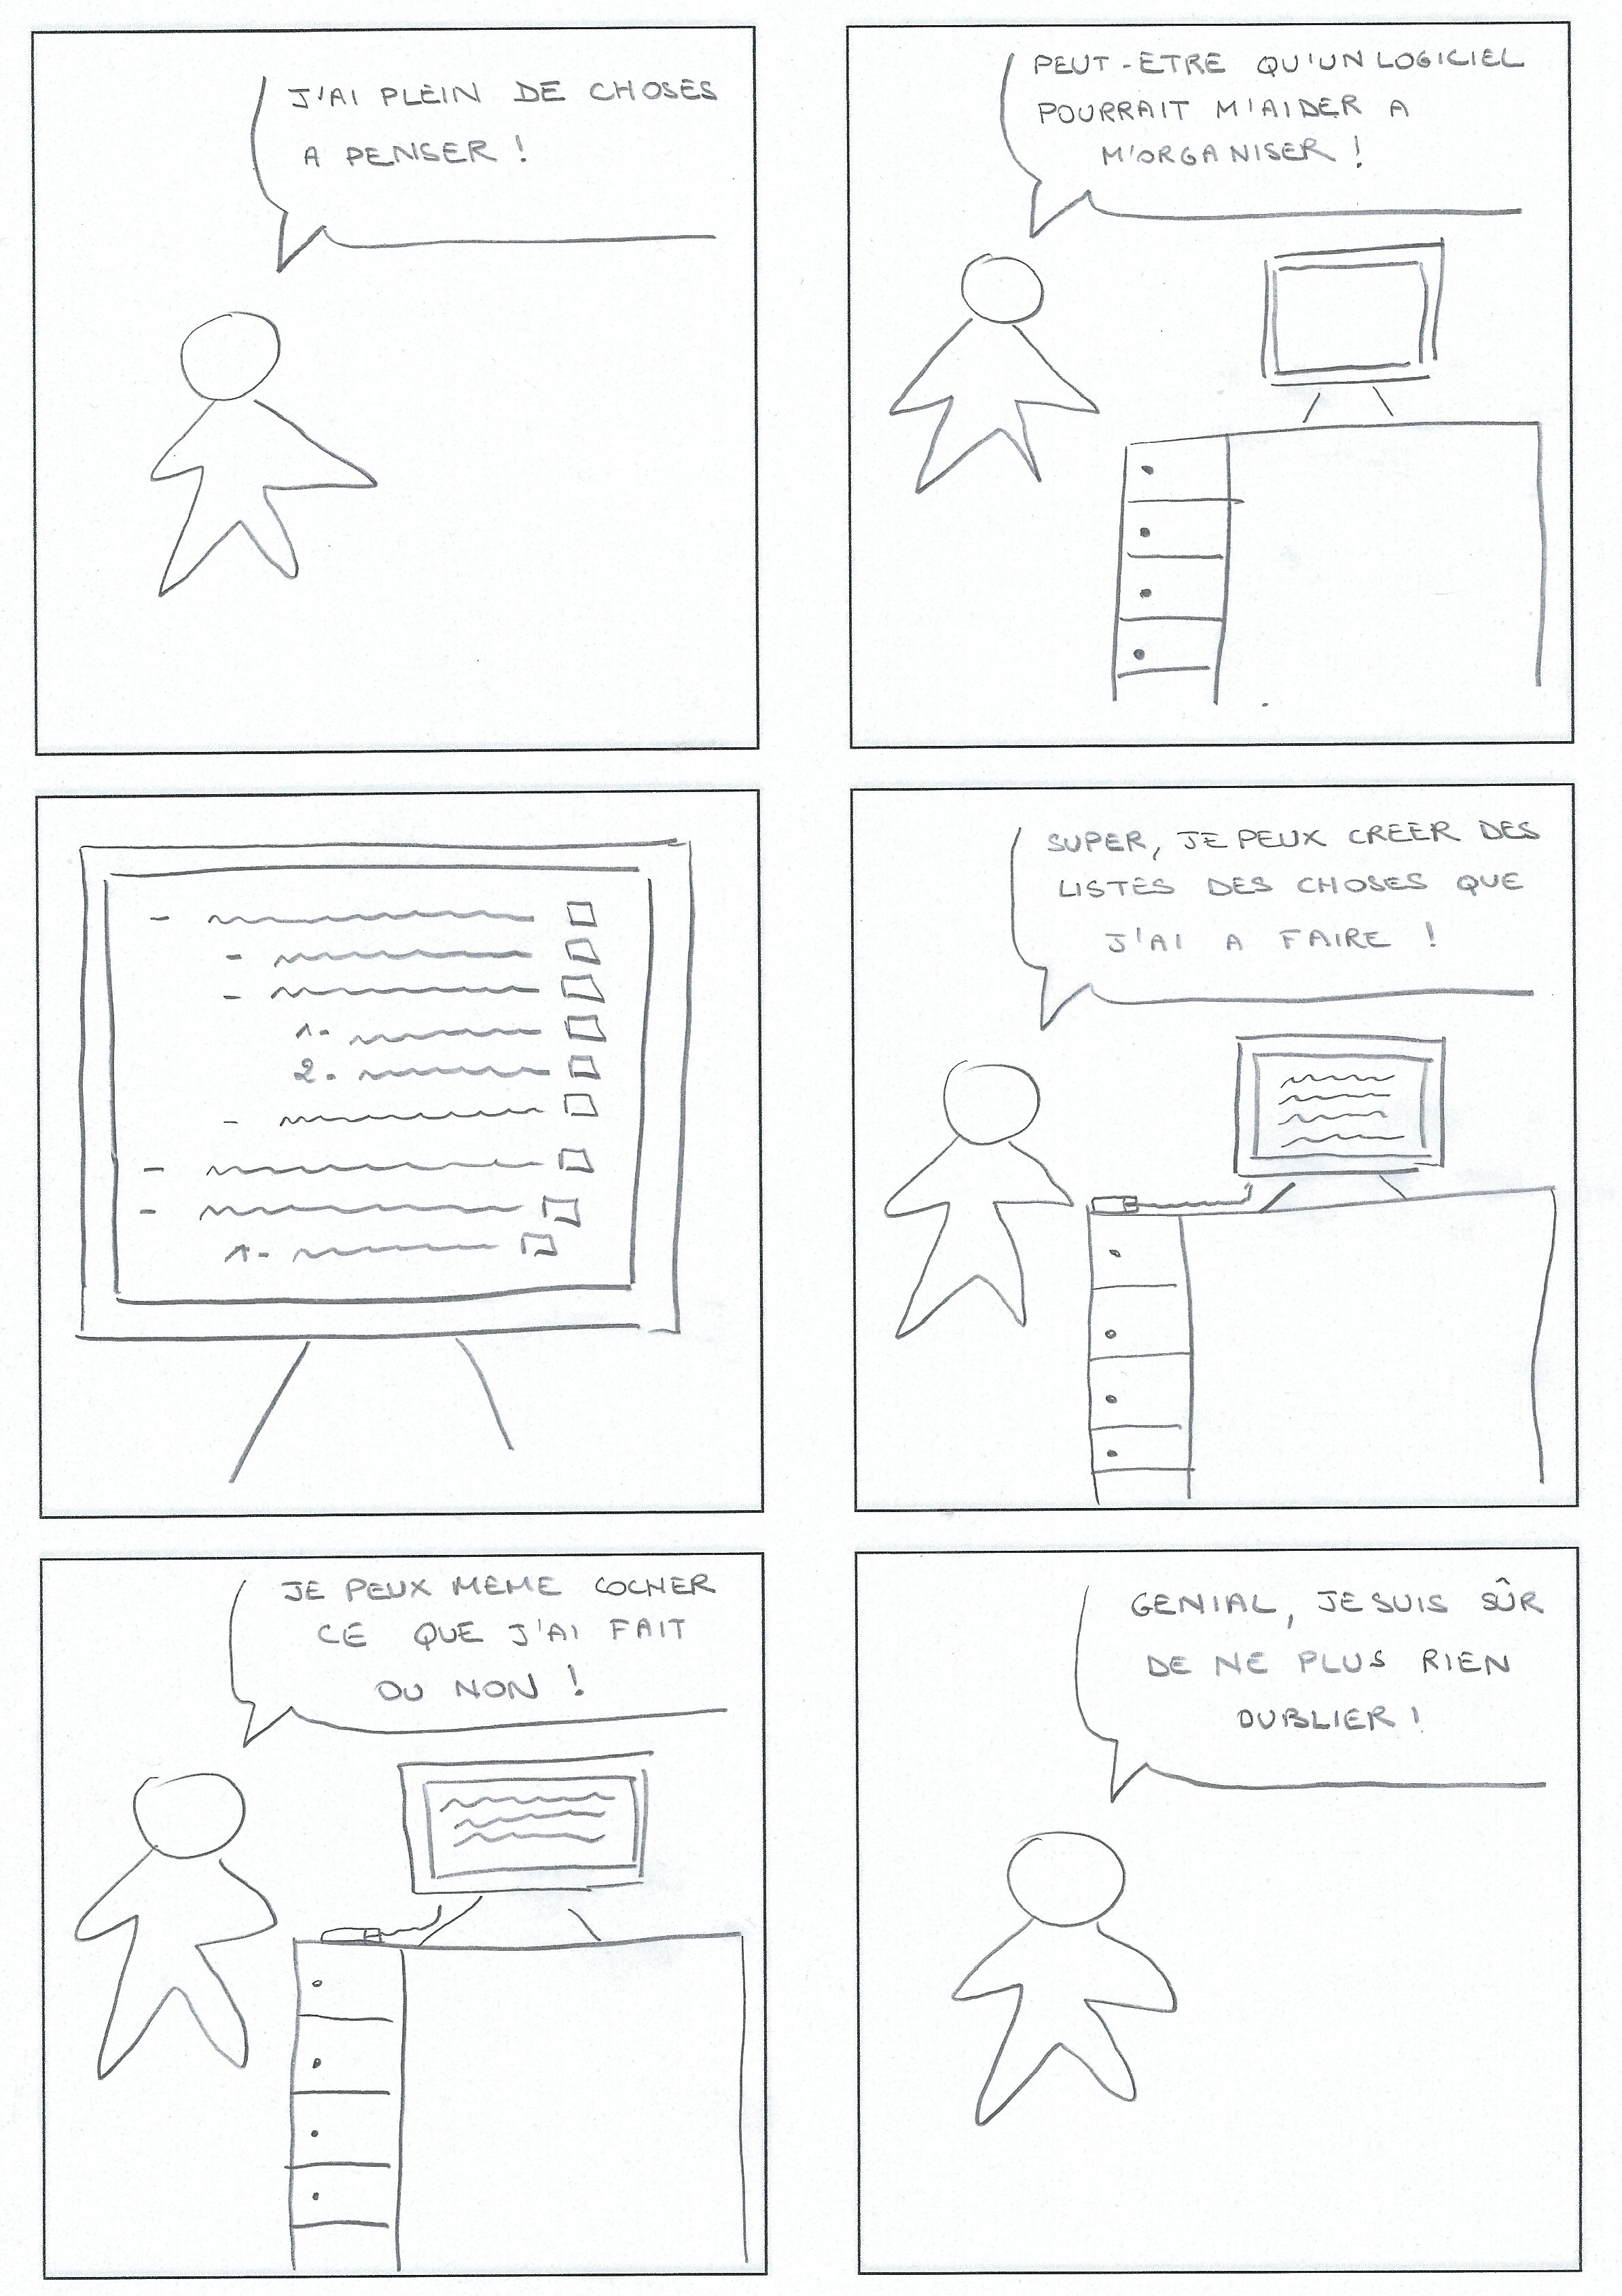
\includegraphics[width=13.9cm]{Images/storyboard.png}
    \caption{Le storyboard}
\end{figure}


\subsection{Paper prototyping}

\subsubsection{Les maquettes}
Voici quelques unes des maquettes réalisées pour le paper prototyping. Les maquettes
ici présentent sont celles qui ont été utilisées pour la réalisation de la vidéo du scénario 1 présenté ci-dessous.
(Lien de la vidéo: \url{http://www.youtube.com/watch?v=YZNYNd3XAL4}).
\begin{figure}[H]
    \center
    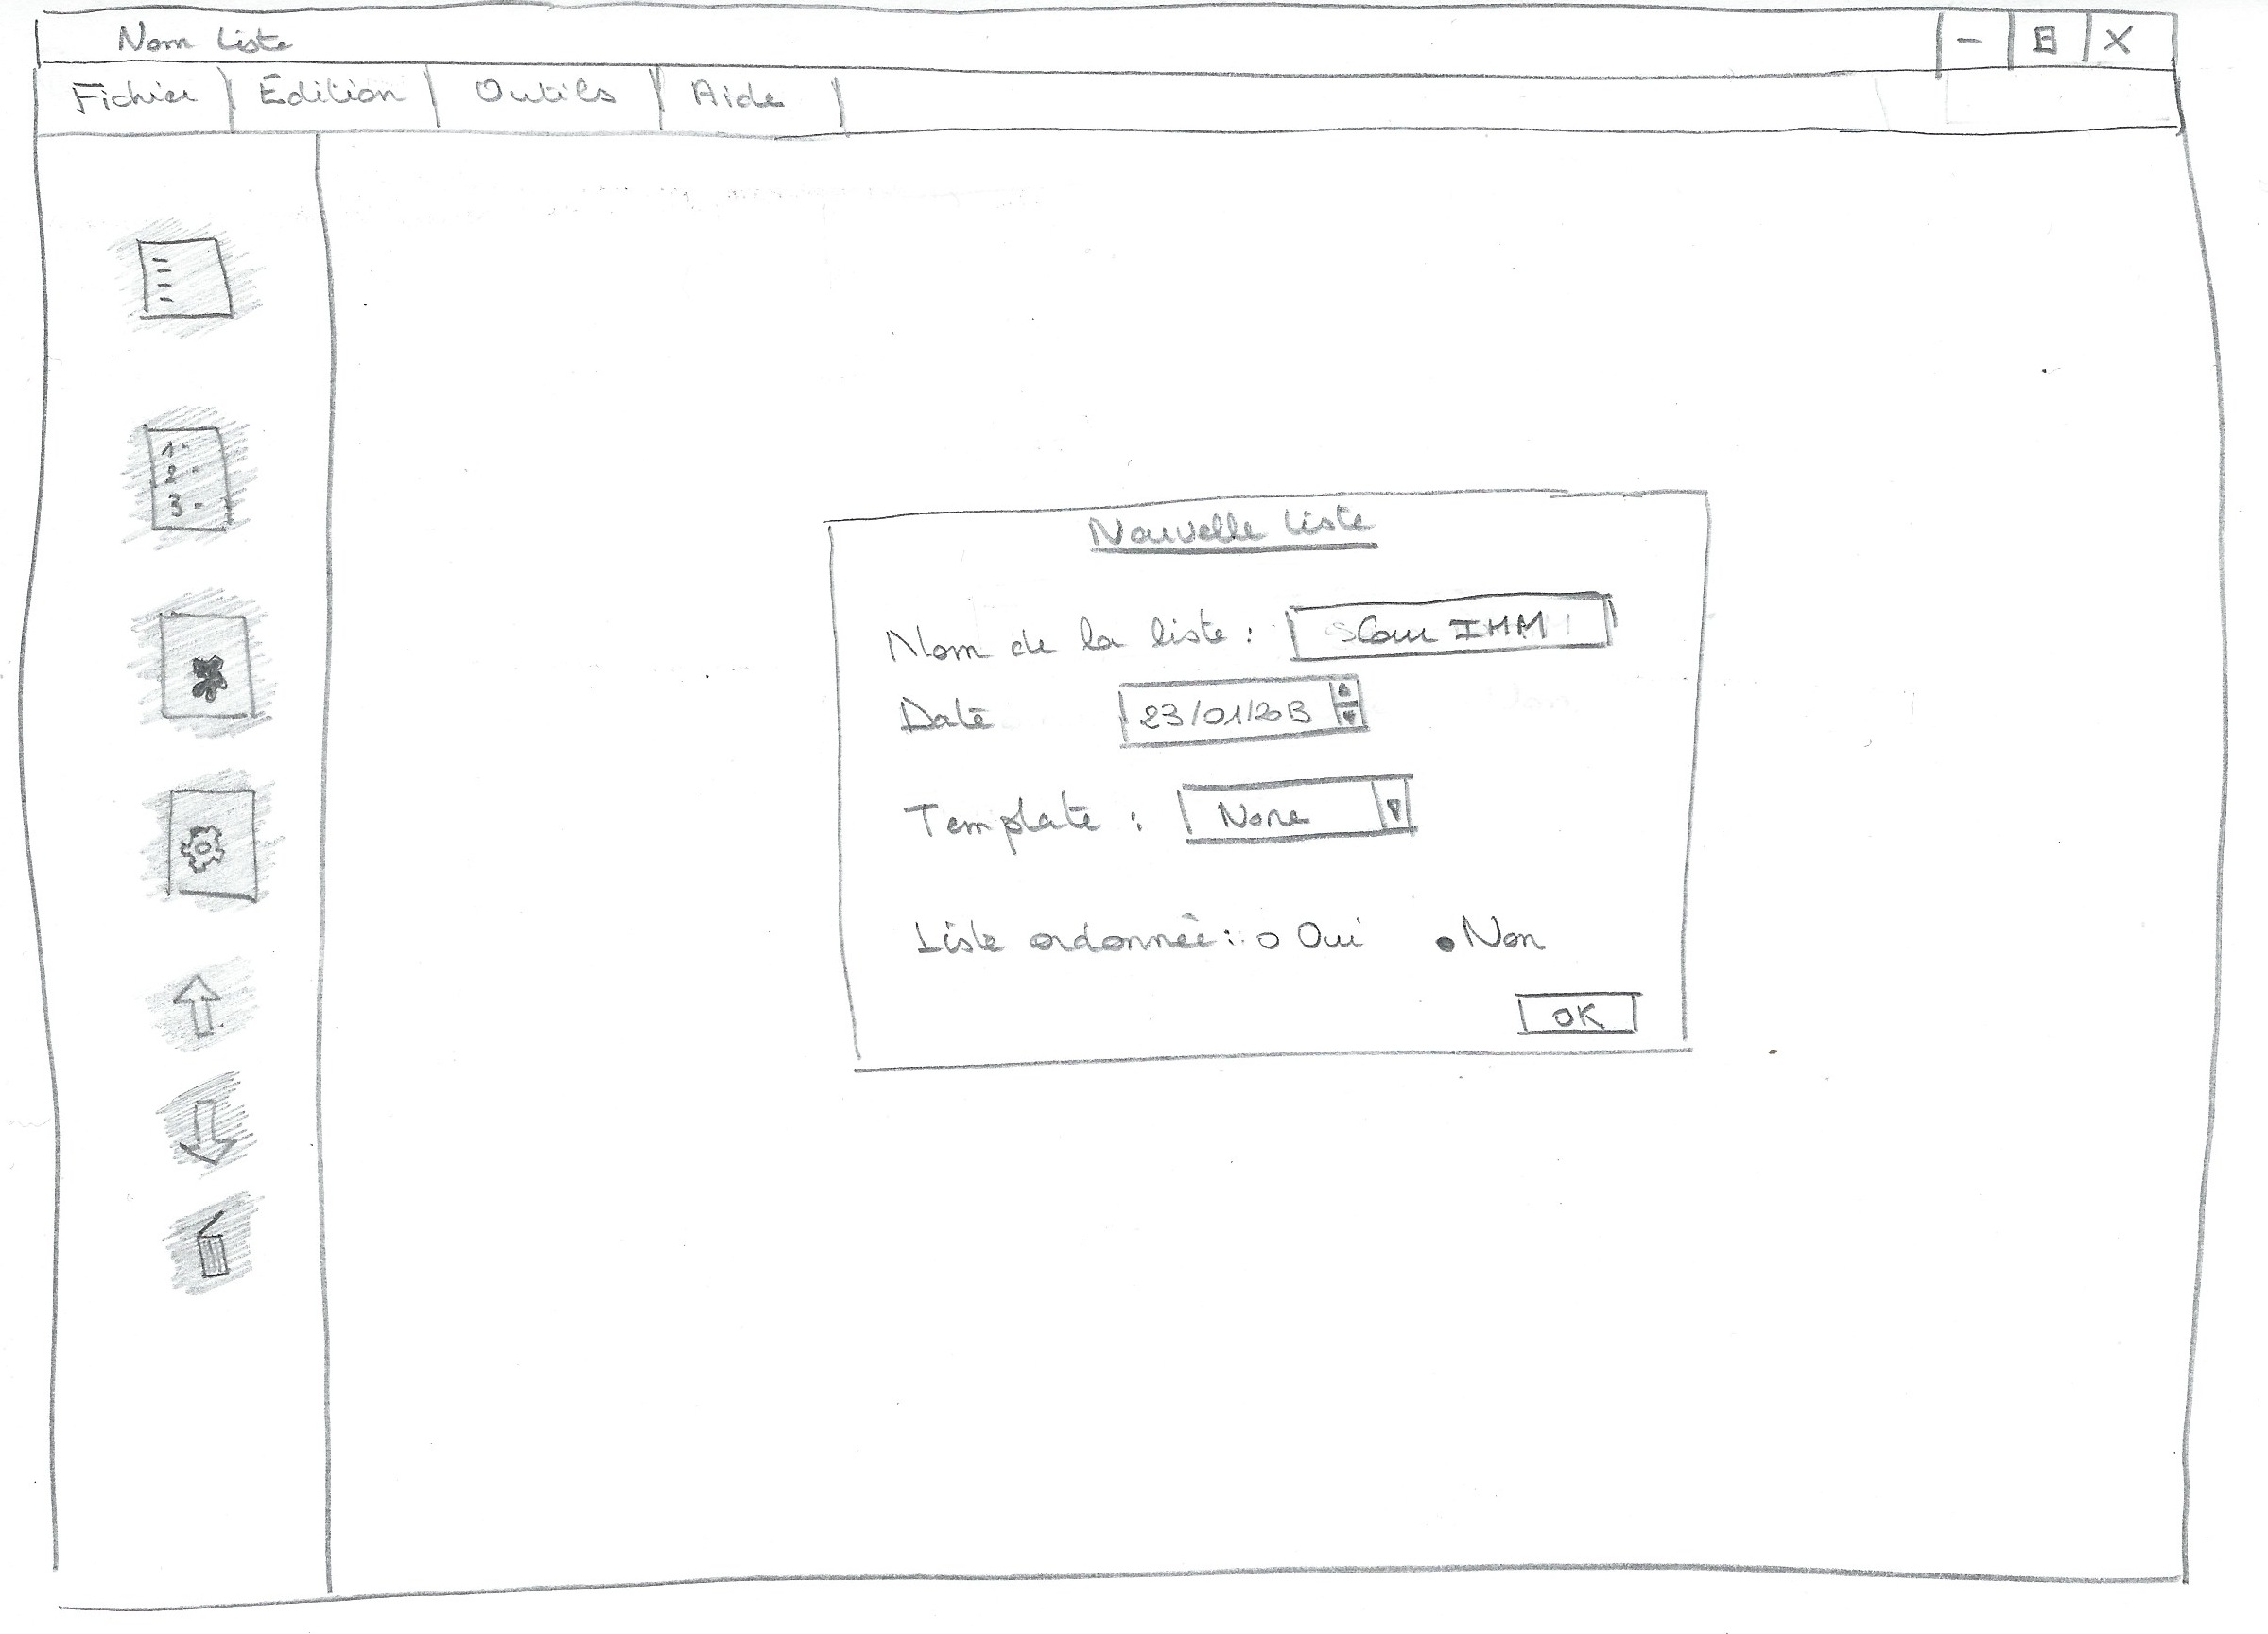
\includegraphics[width=6.8cm]{Images/maquette1.jpeg}
    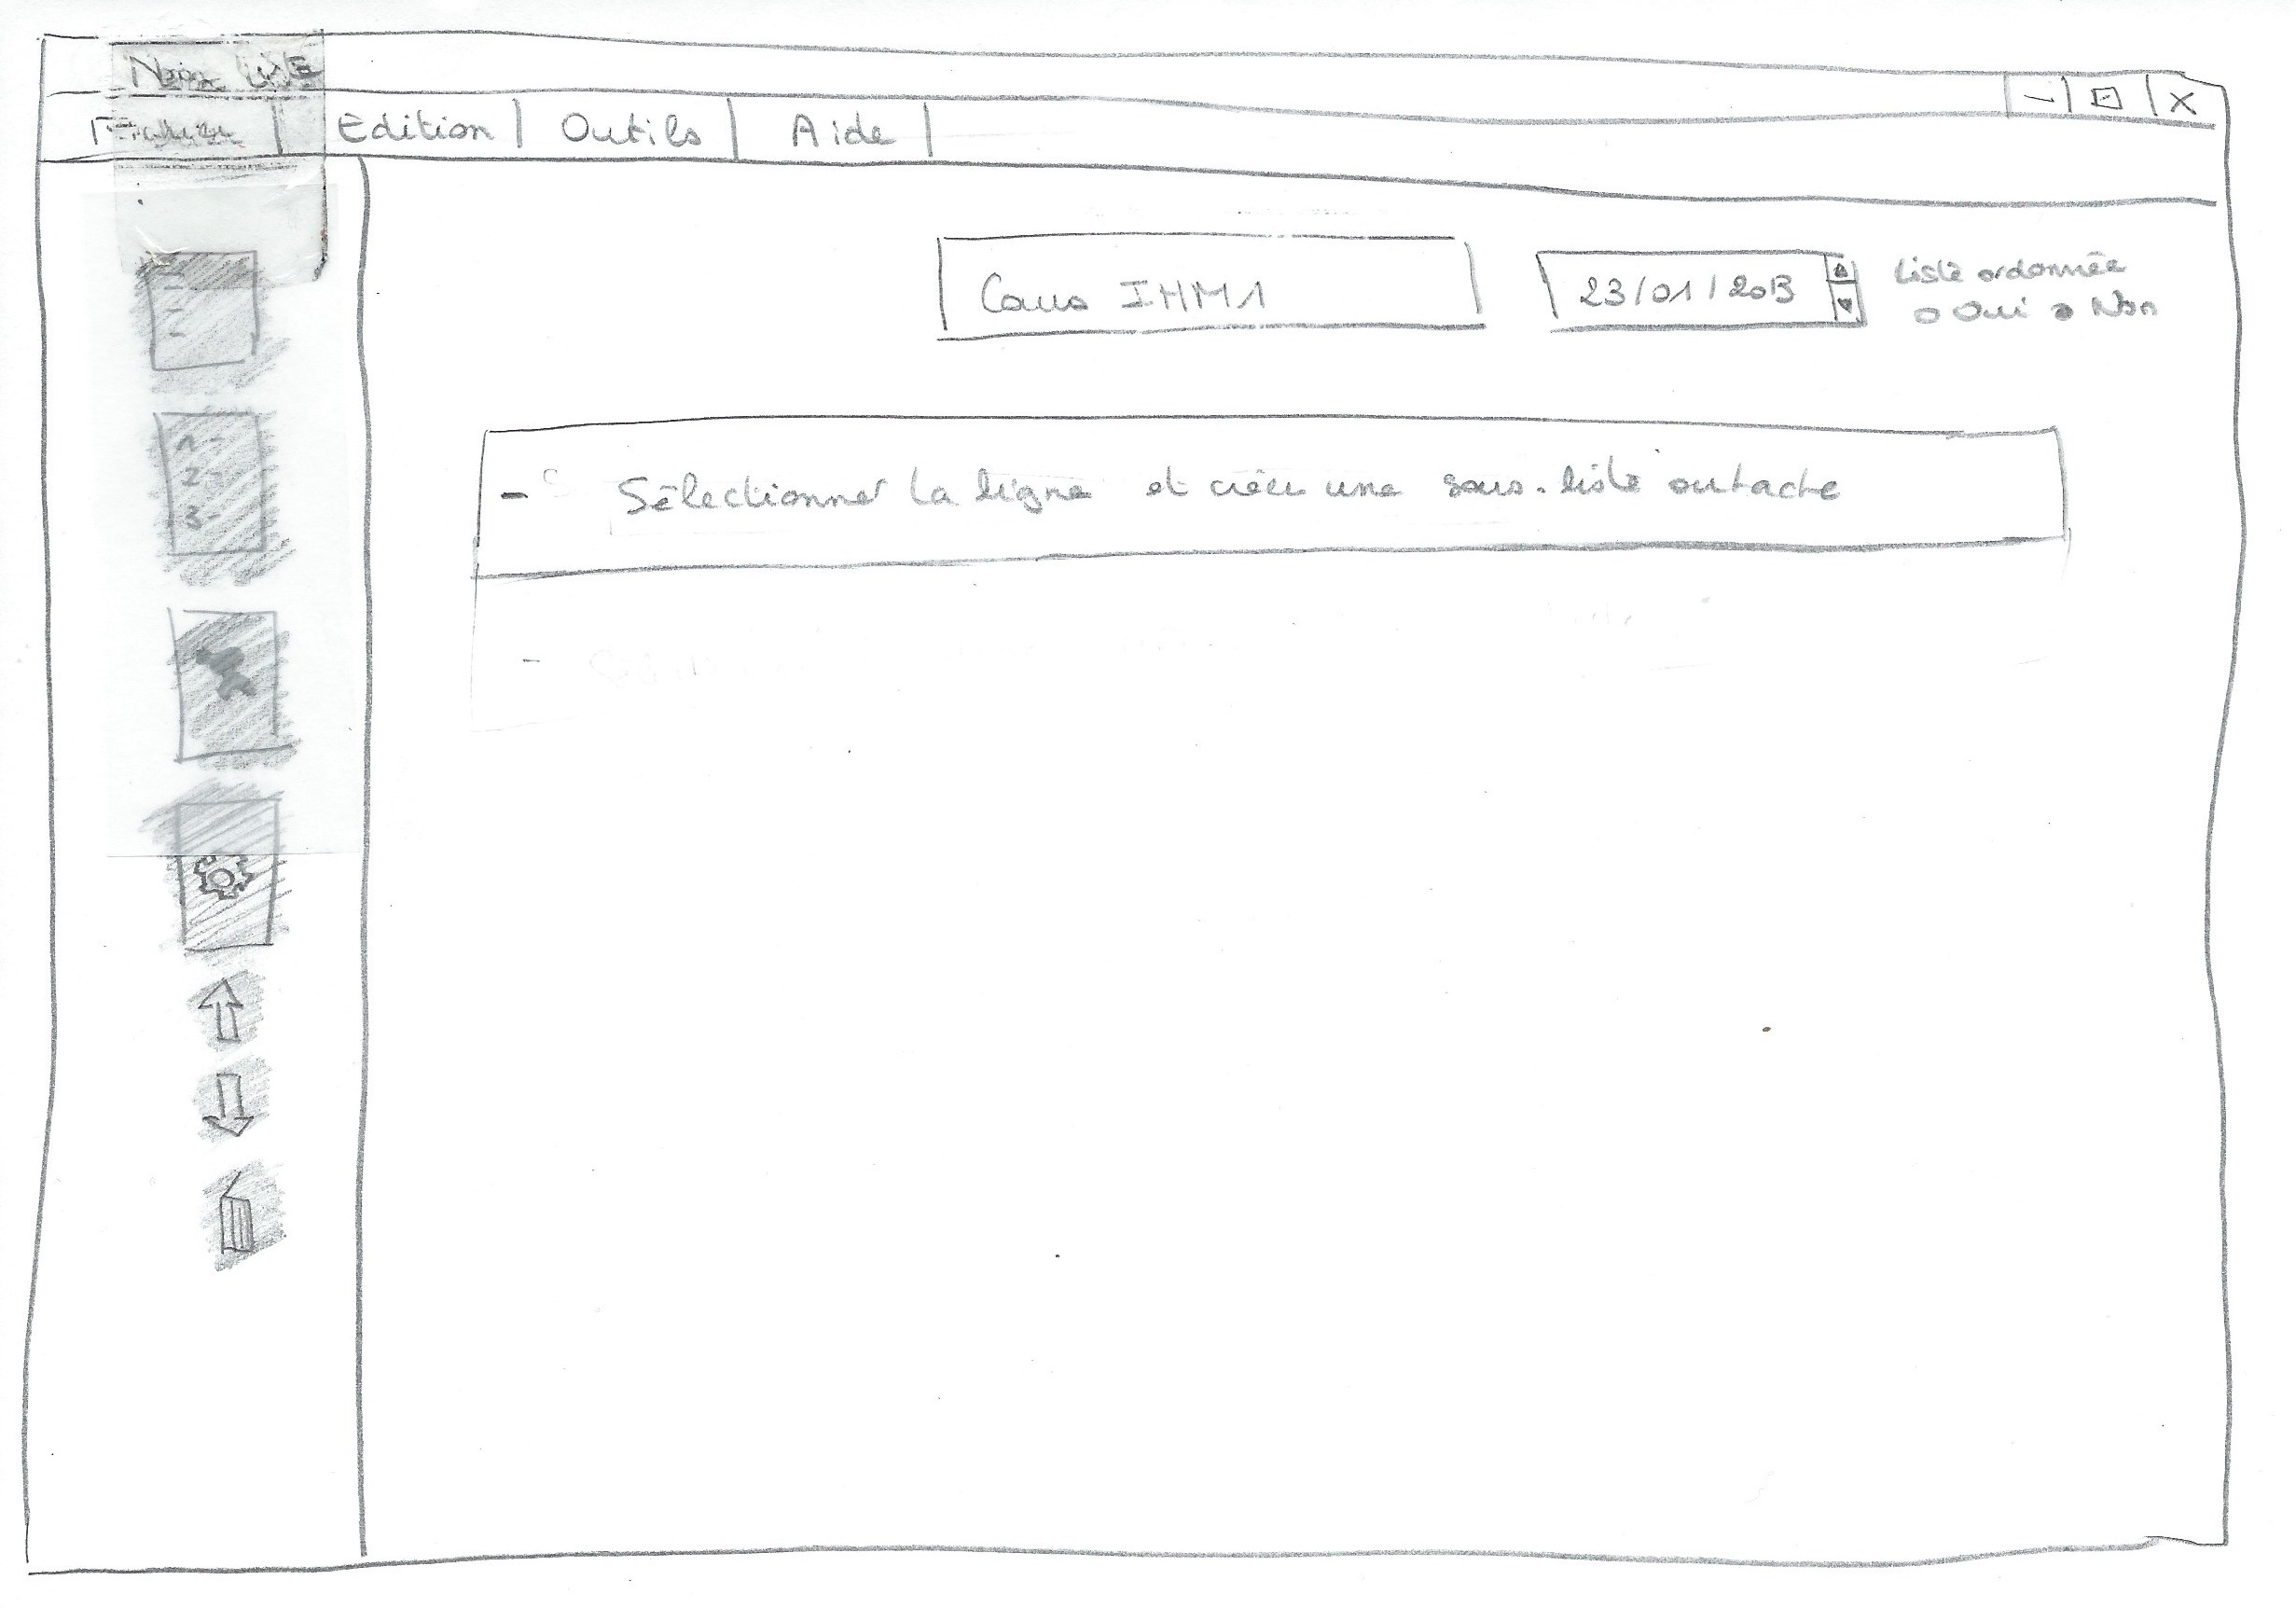
\includegraphics[width=7.1cm]{Images/maquette2.jpeg}
    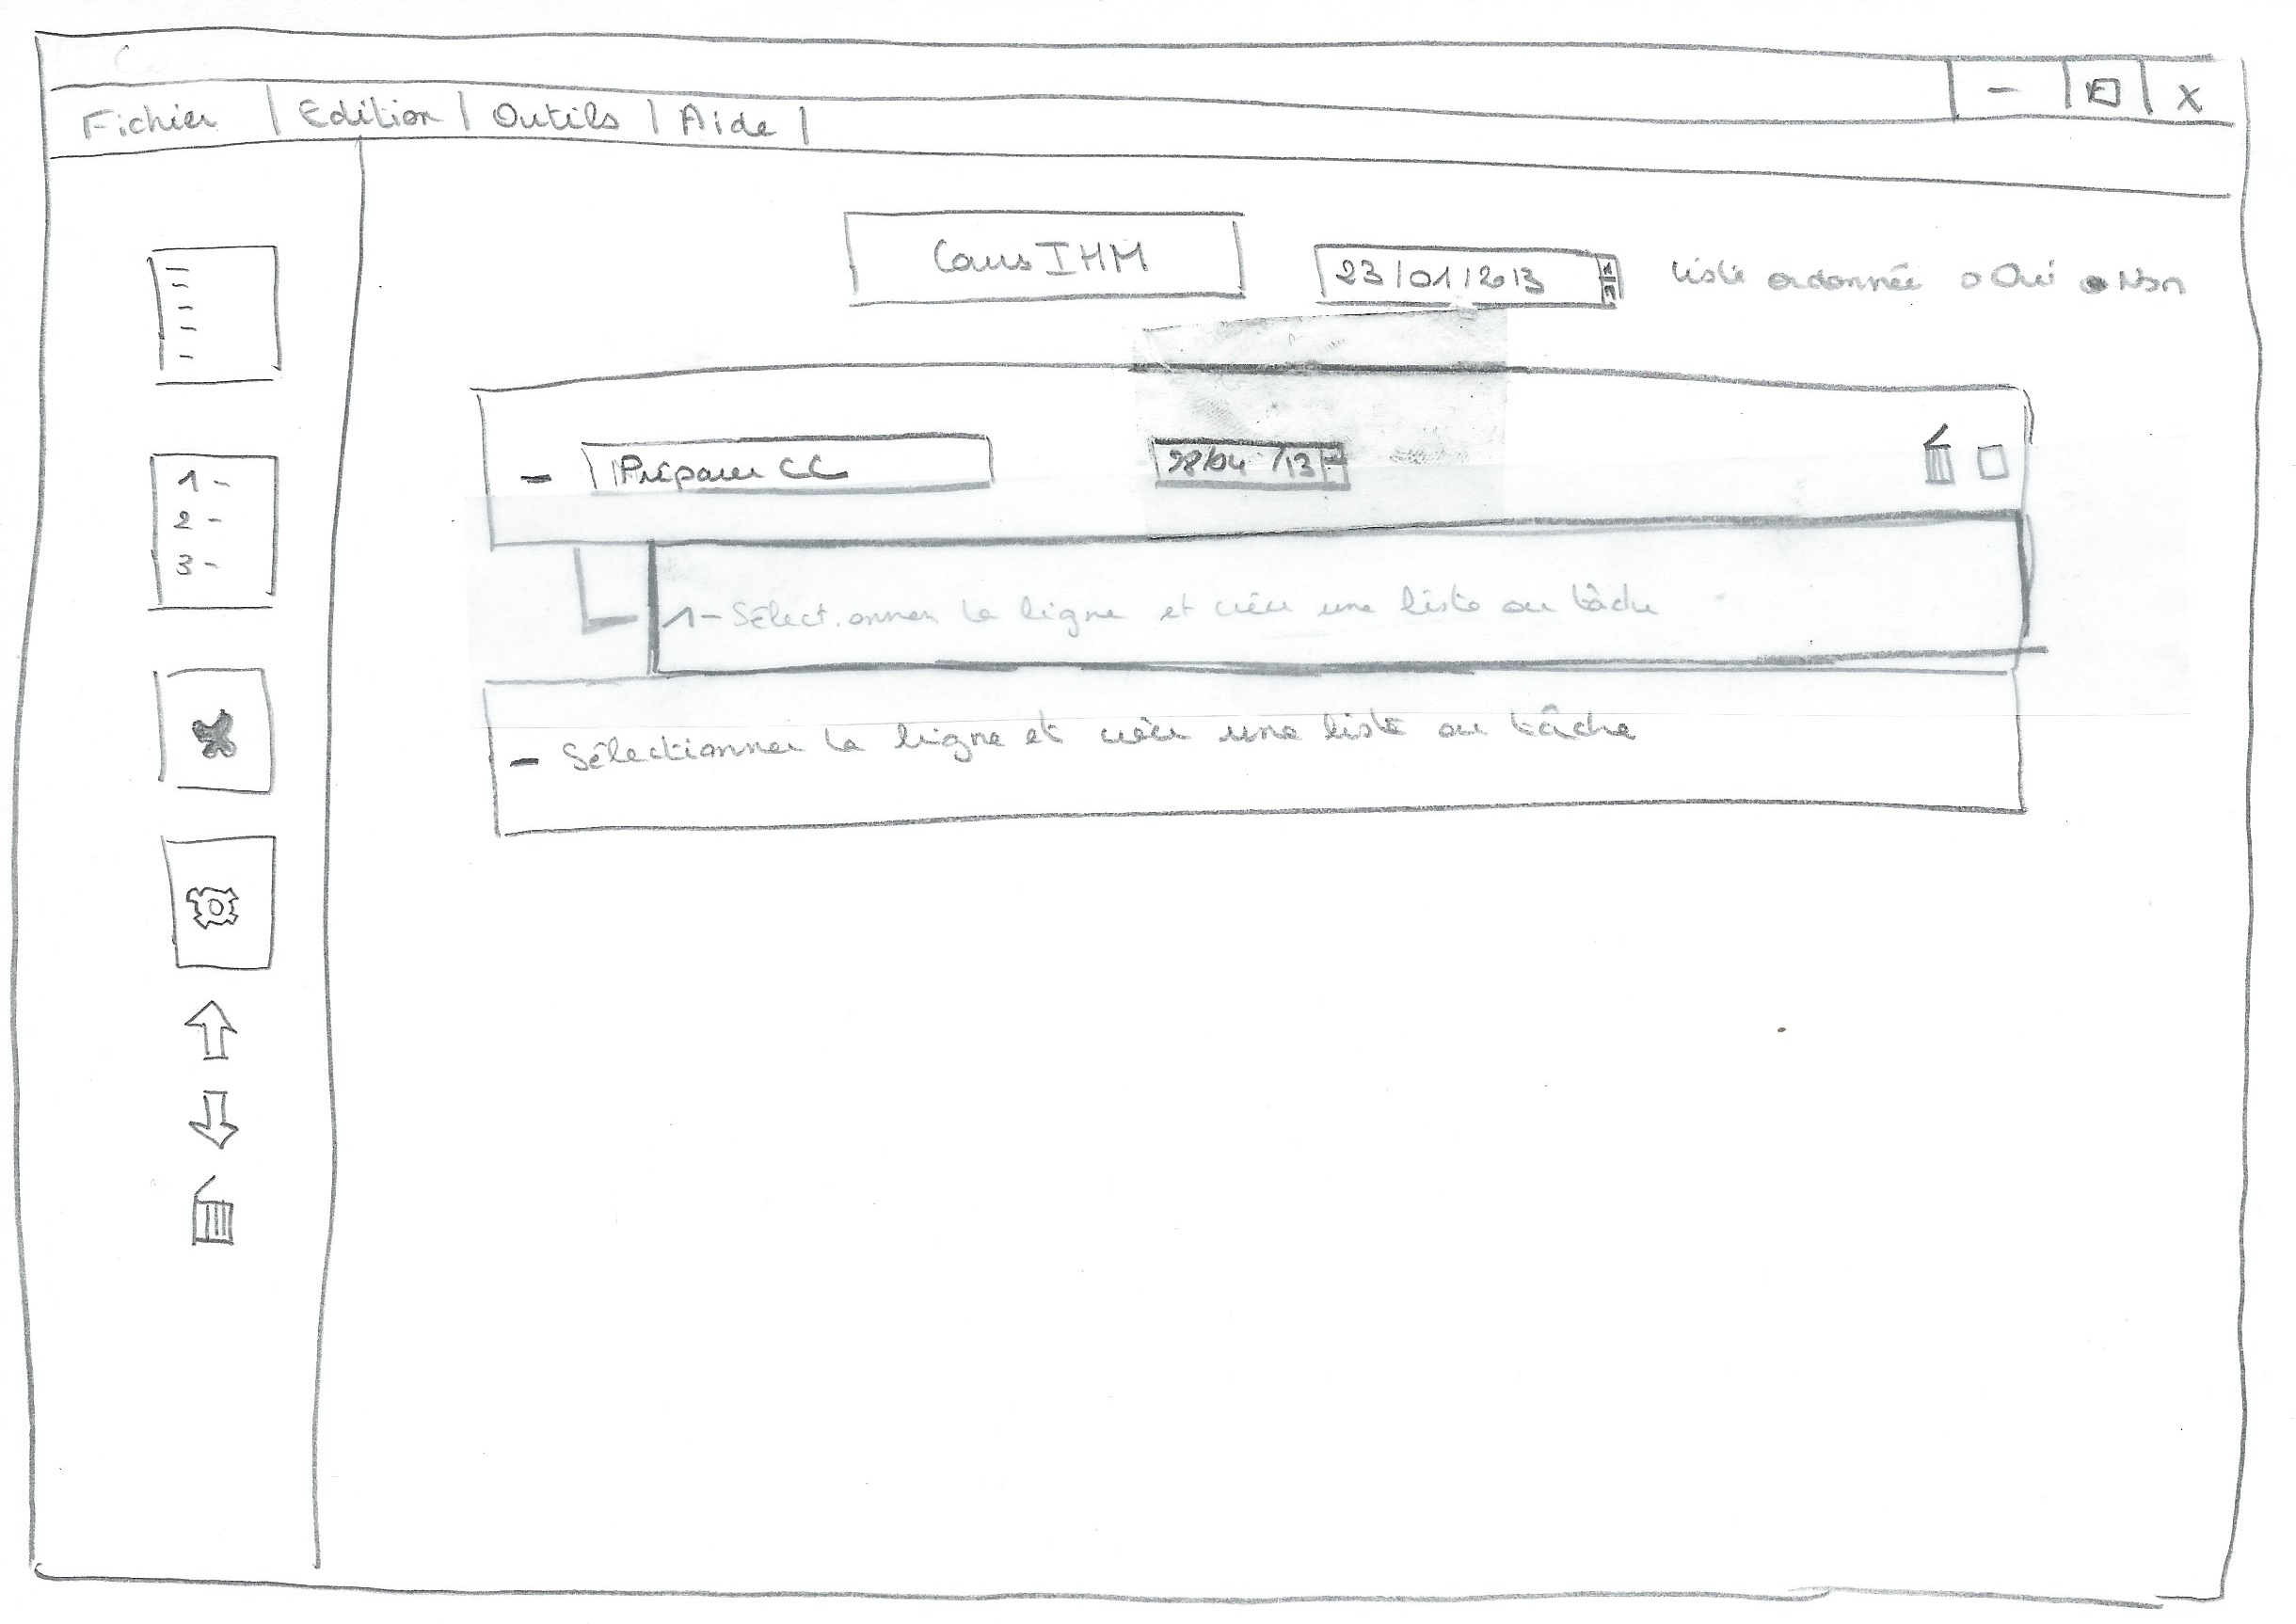
\includegraphics[width=6.8cm]{Images/maquette3.jpeg}
    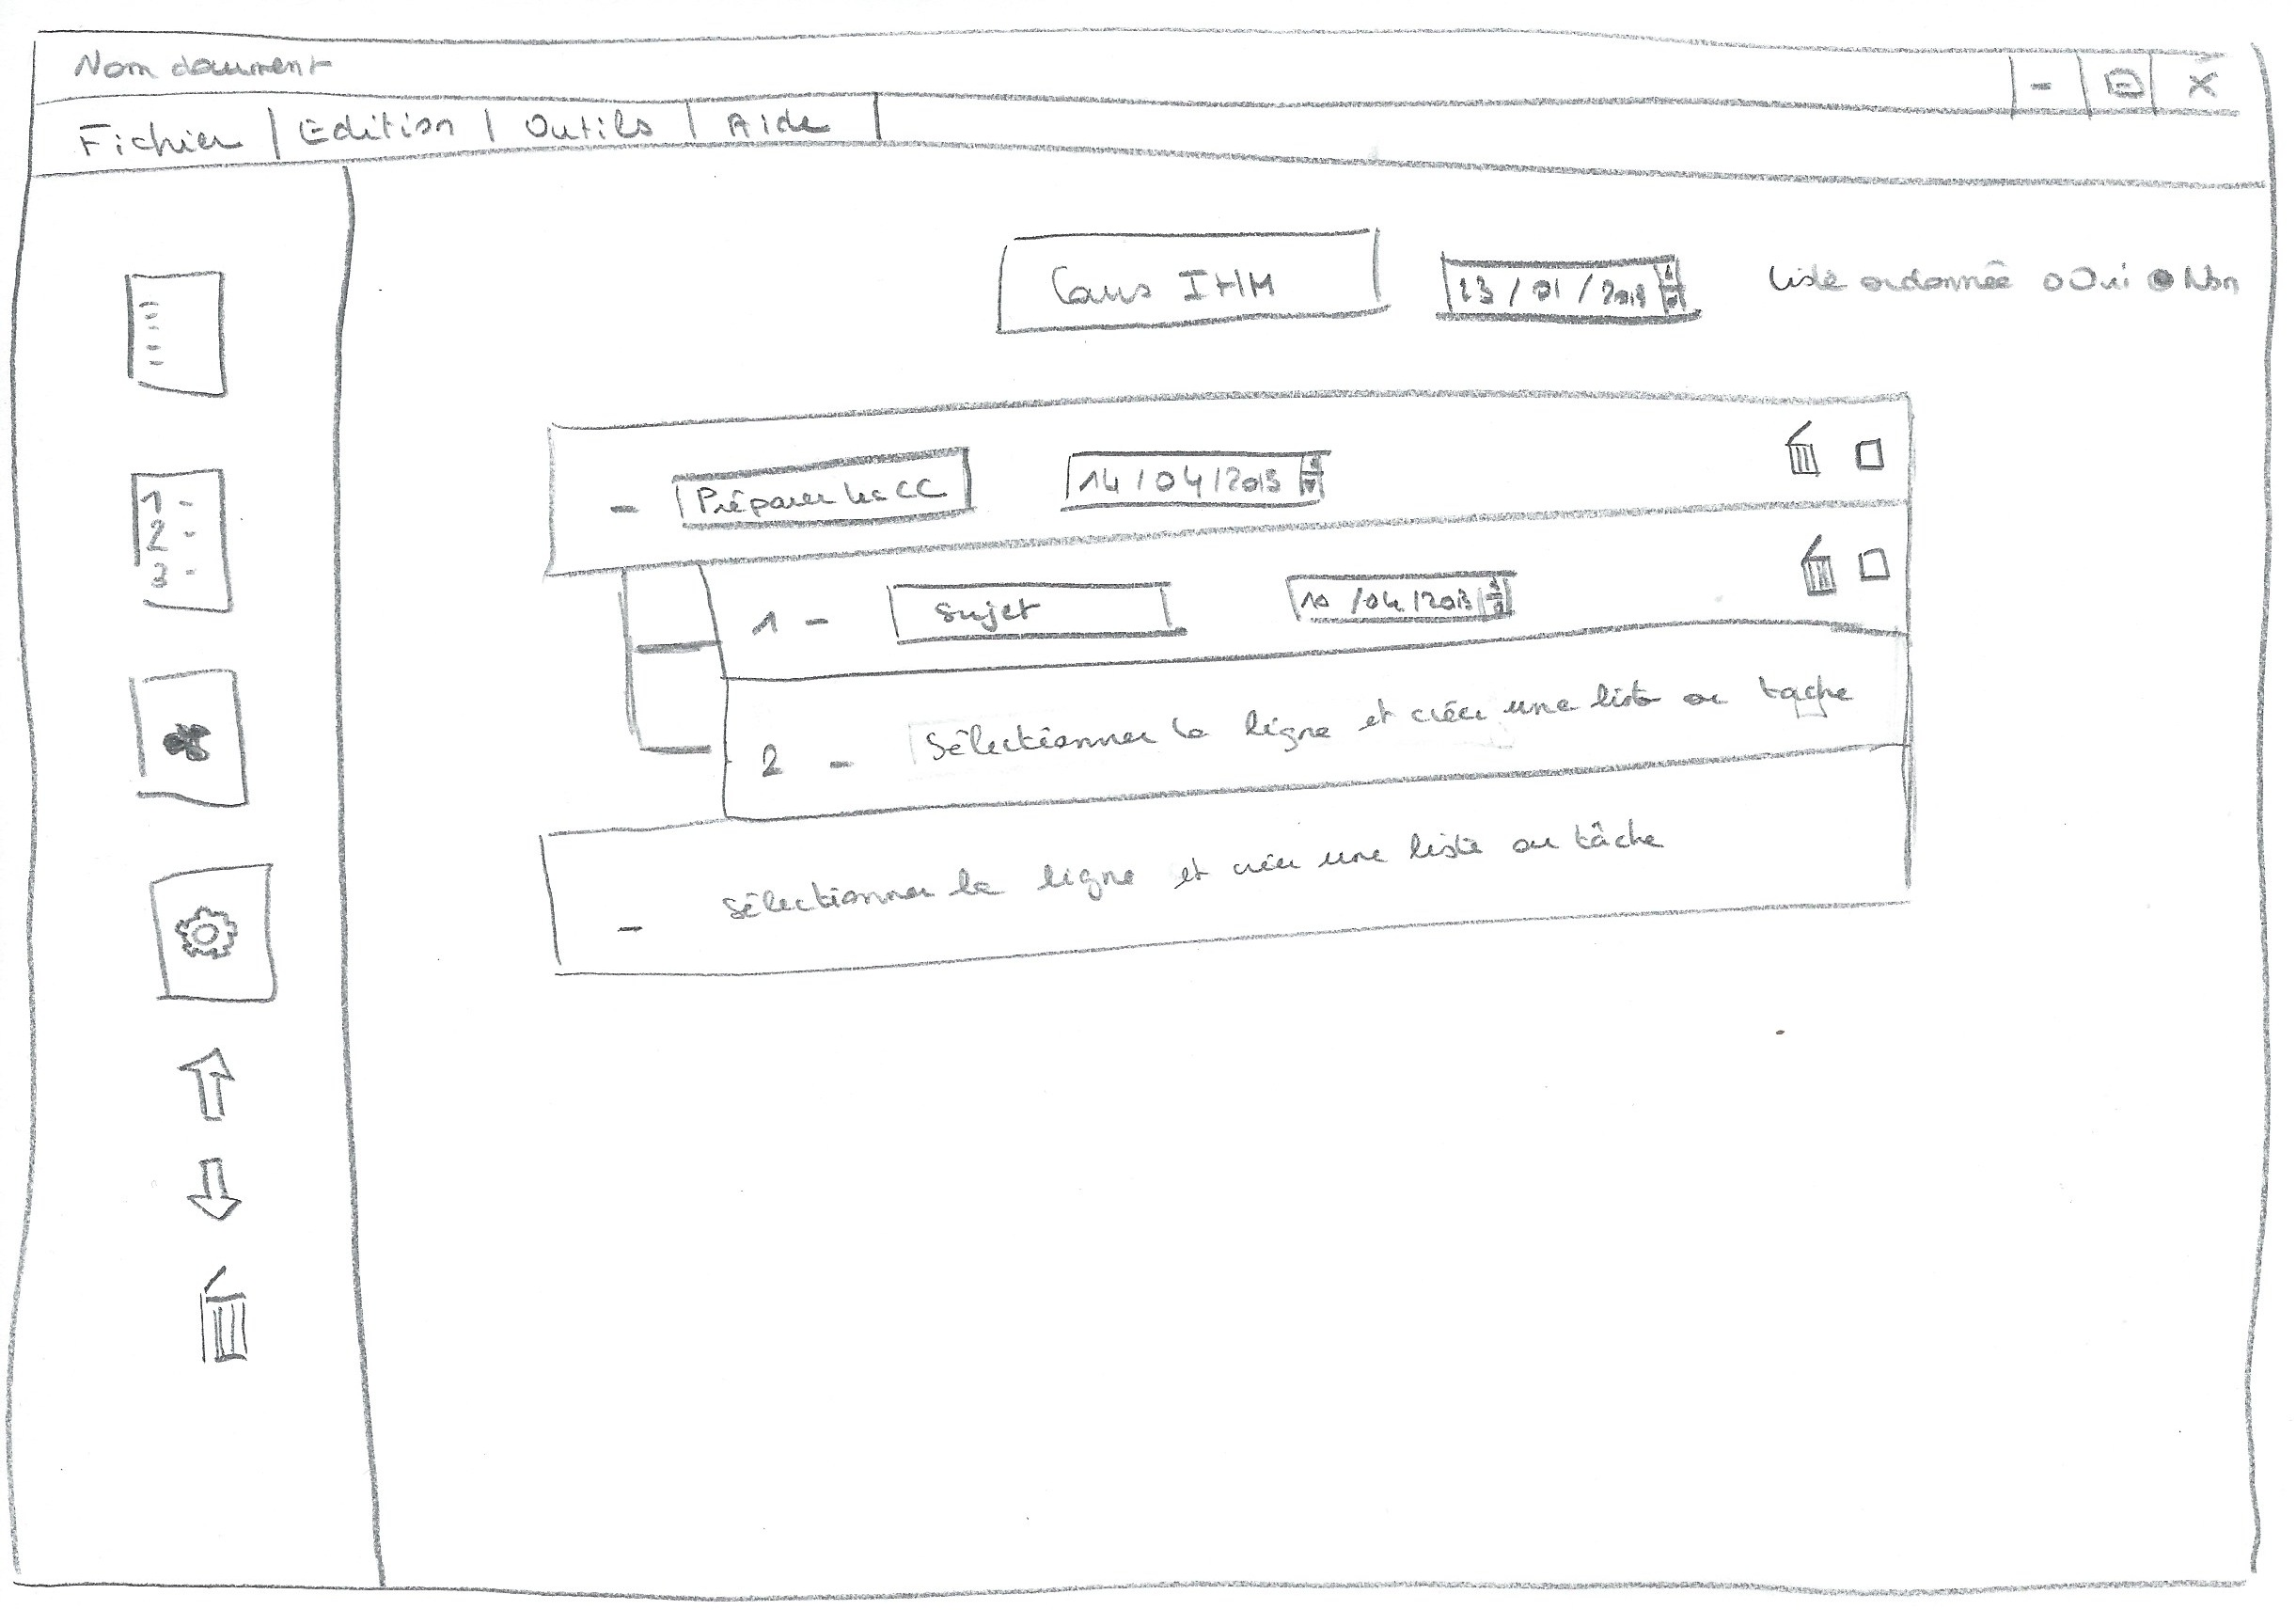
\includegraphics[width=6.8cm]{Images/maquette4.jpeg}
    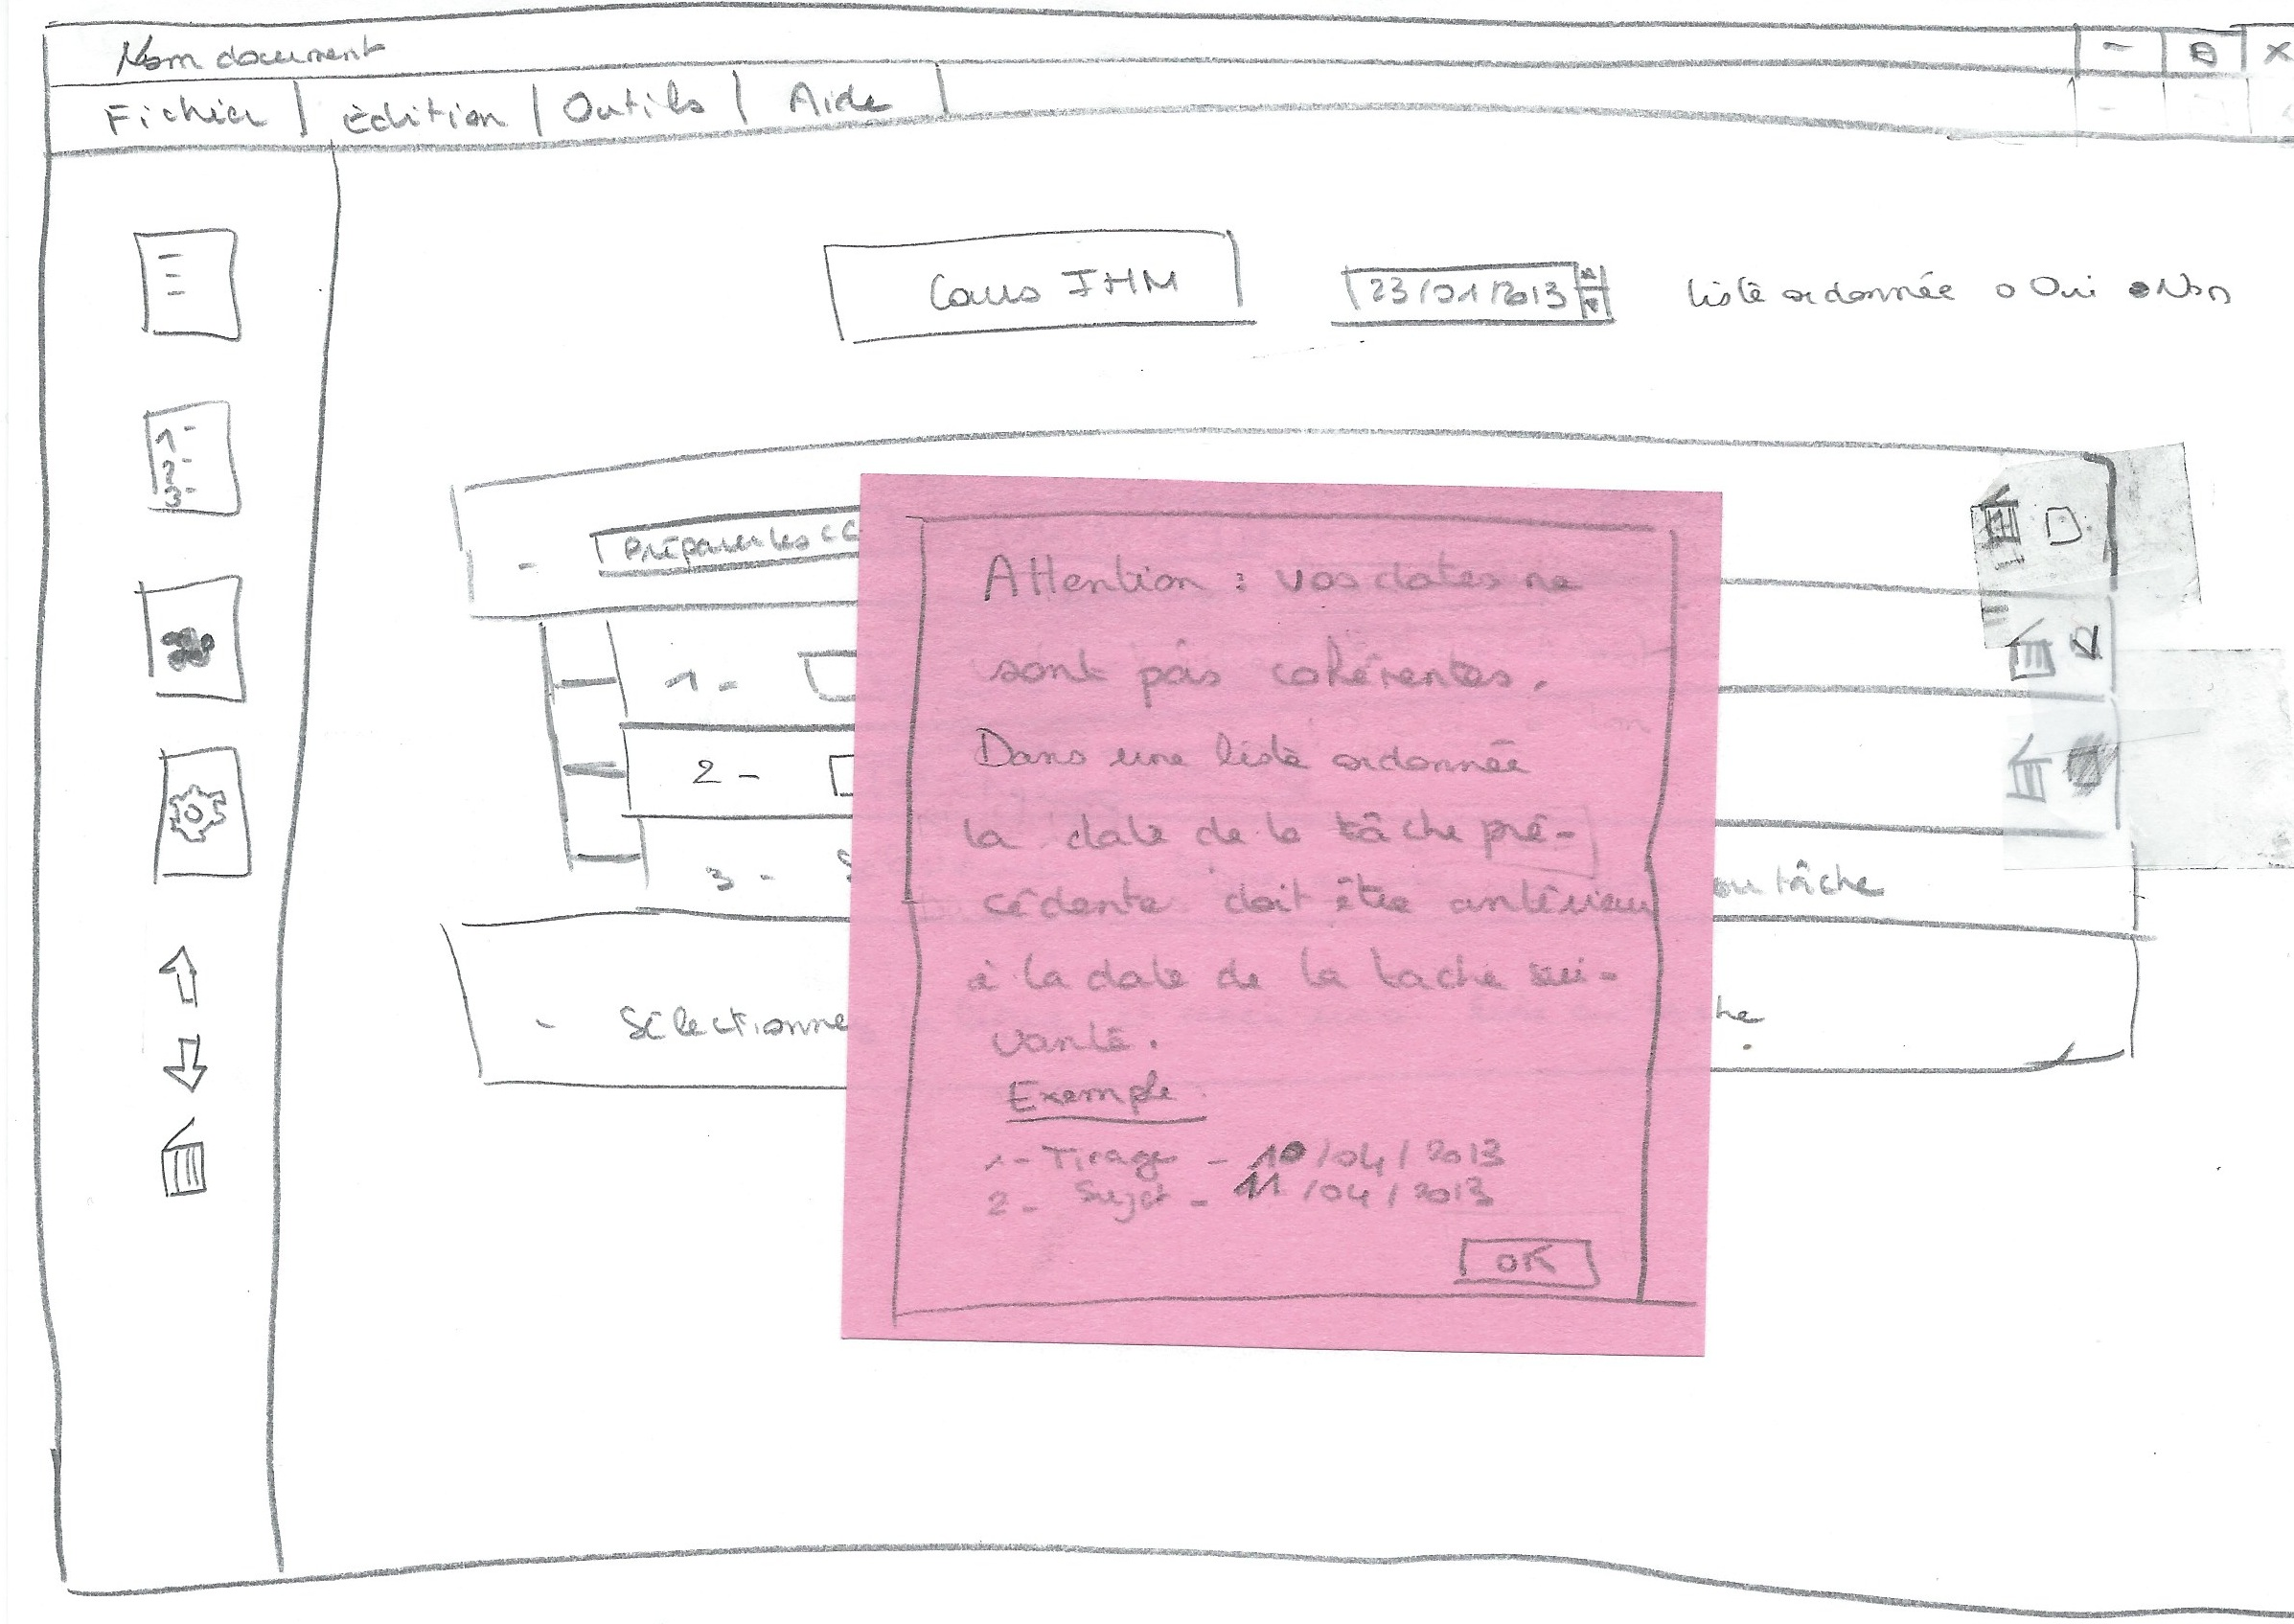
\includegraphics[width=6.8cm]{Images/maquette5.jpeg}
    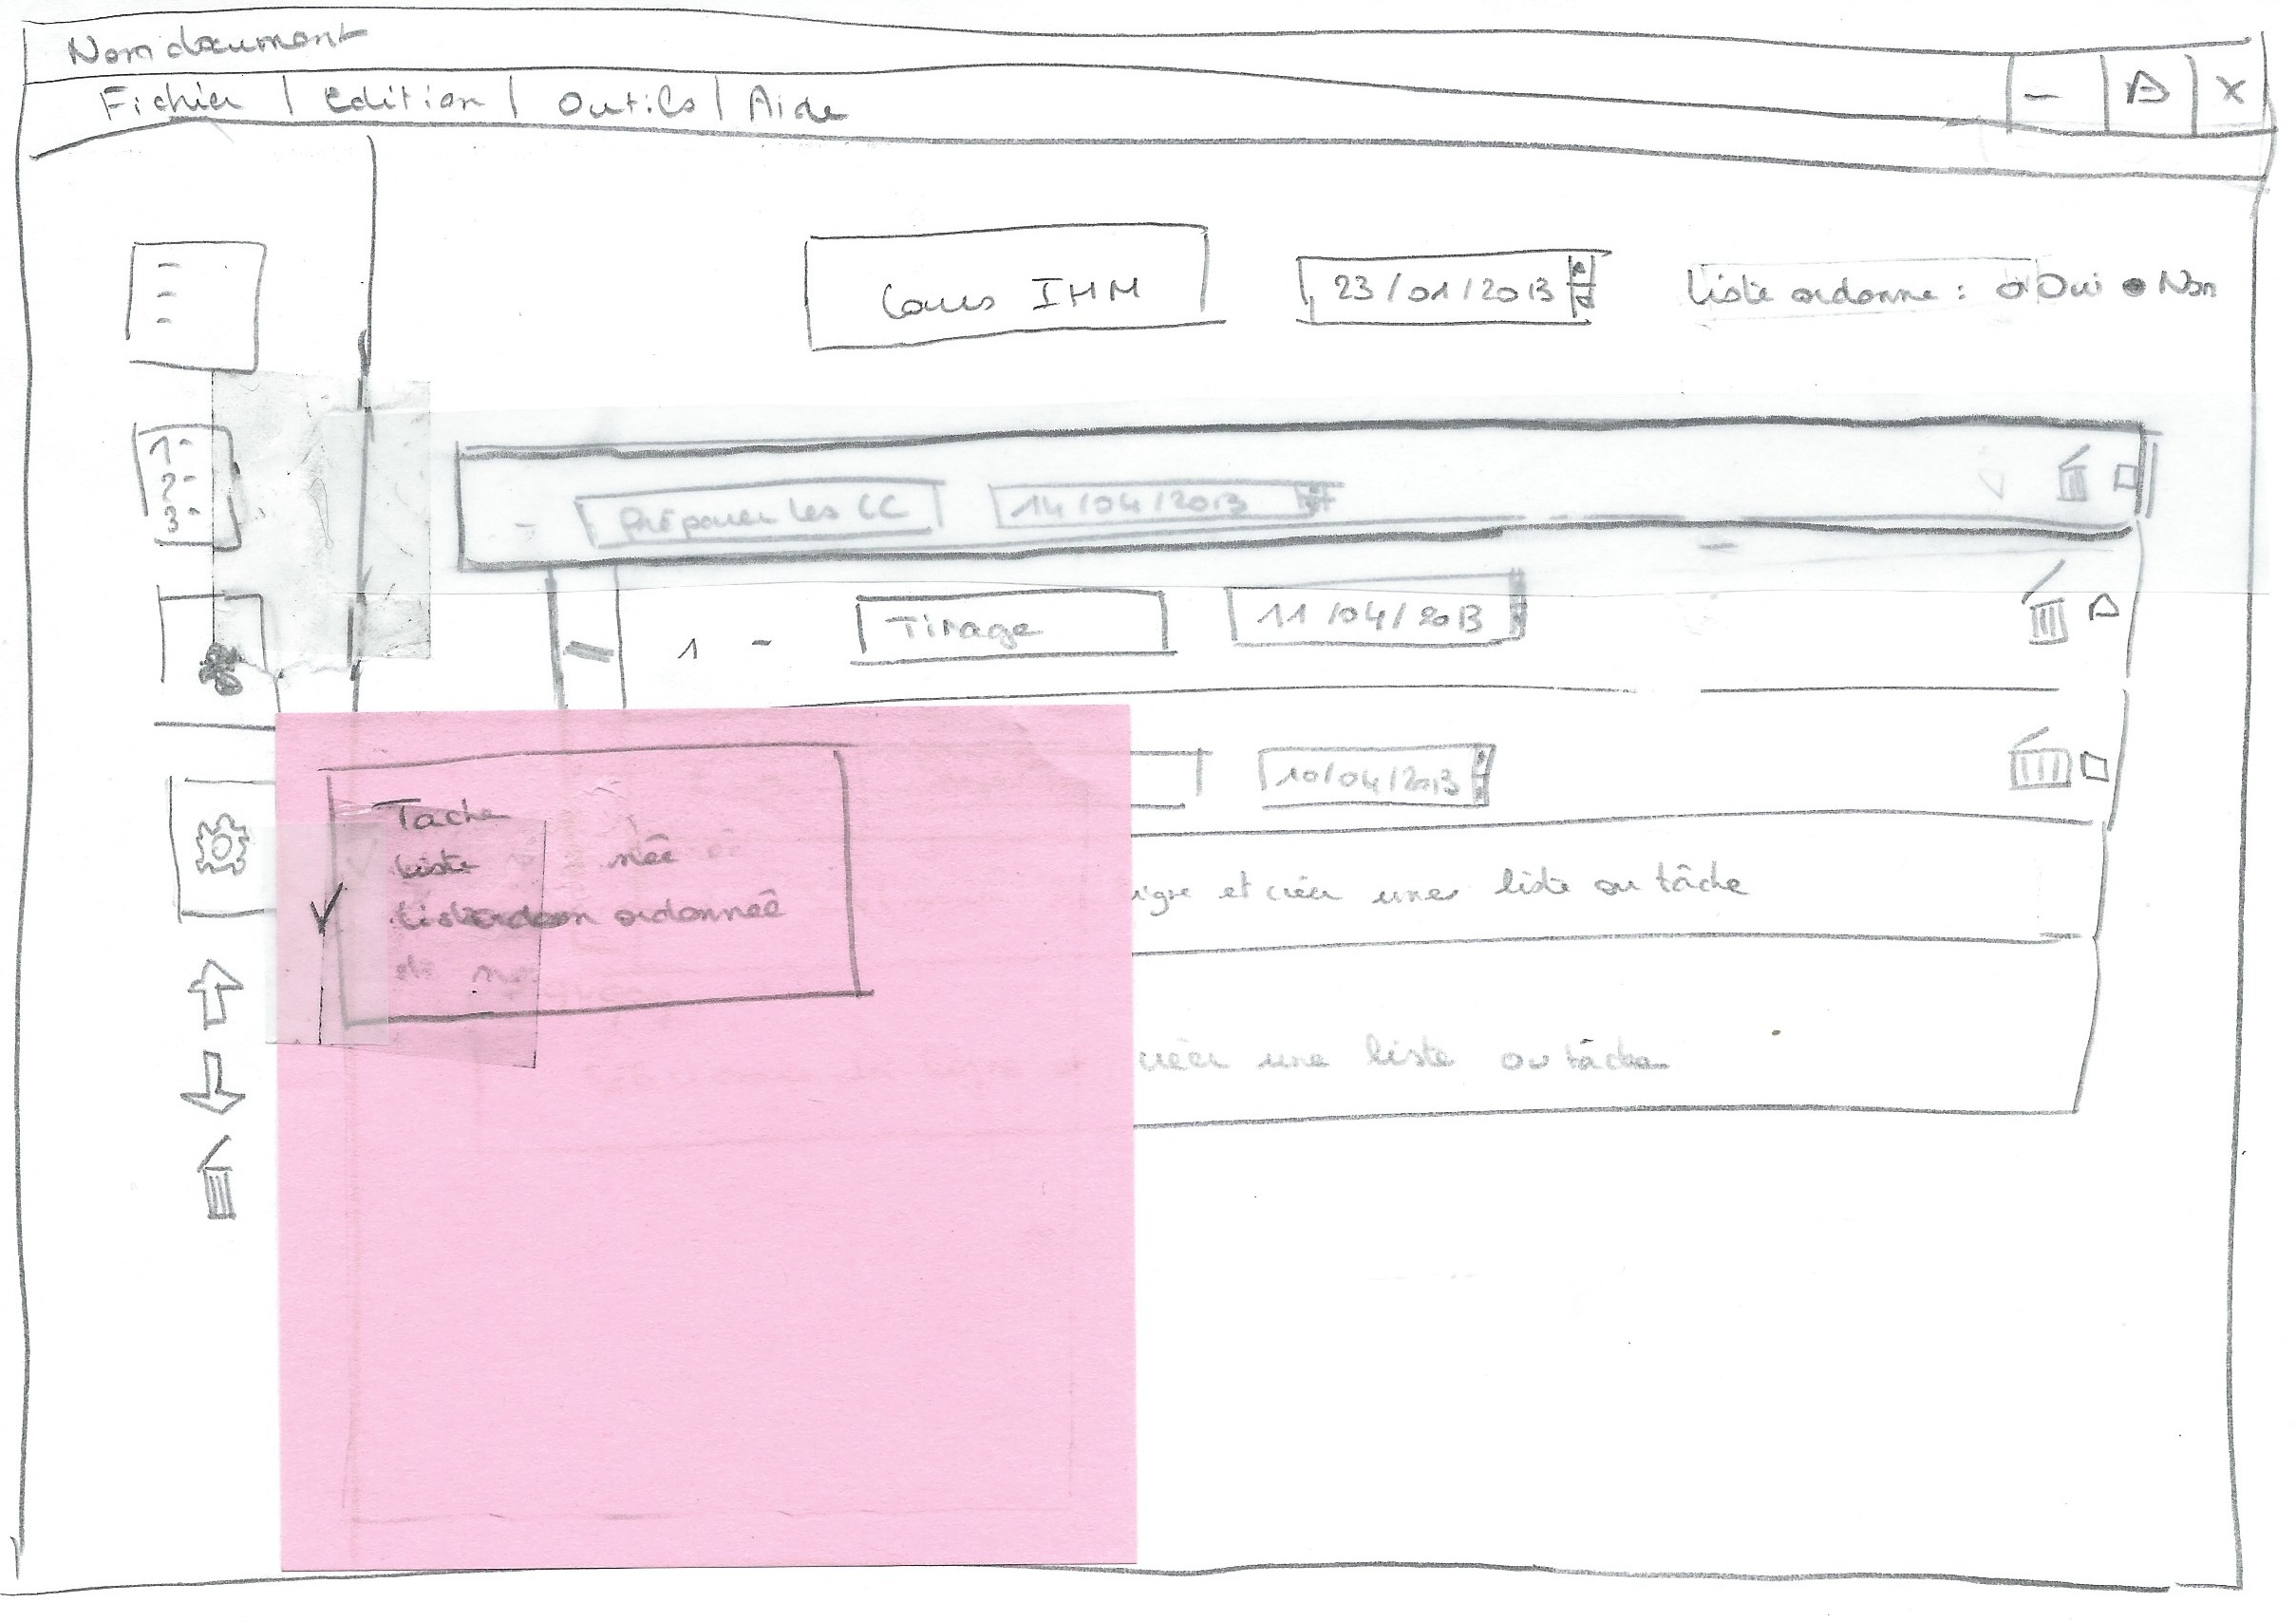
\includegraphics[width=6.8cm]{Images/maquette6.jpeg}
    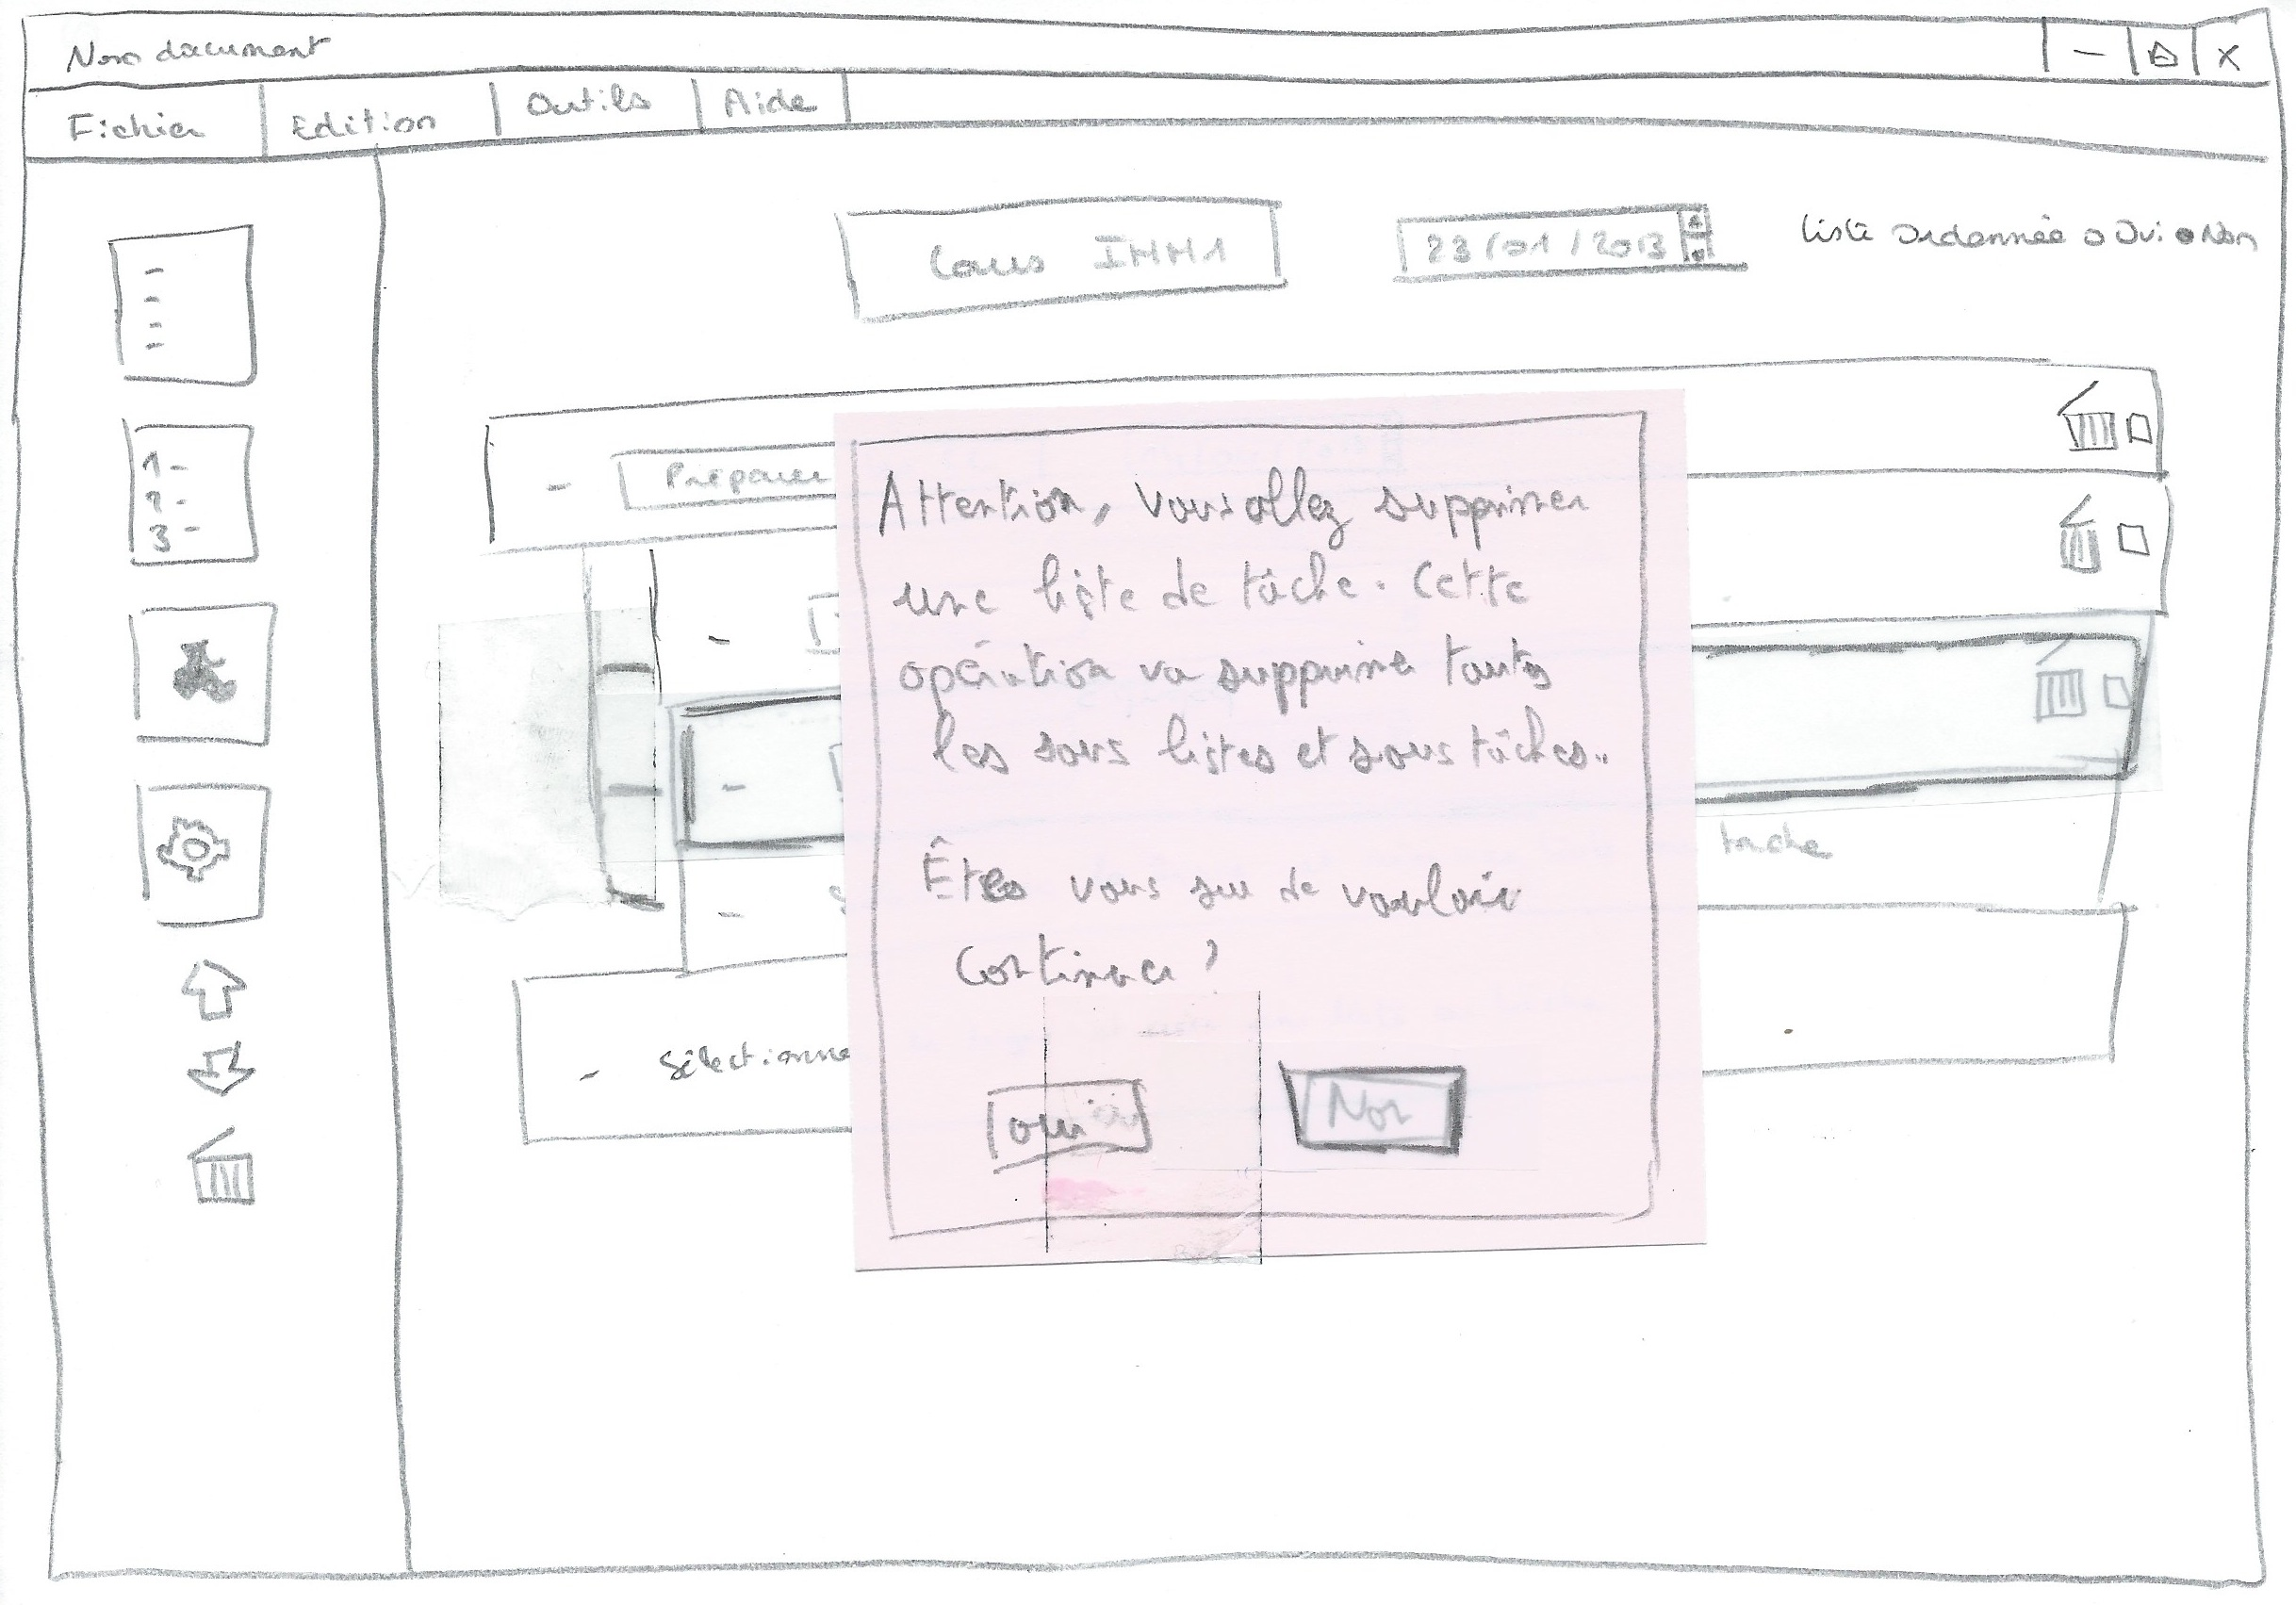
\includegraphics[width=6.8cm]{Images/maquette7.jpeg}
    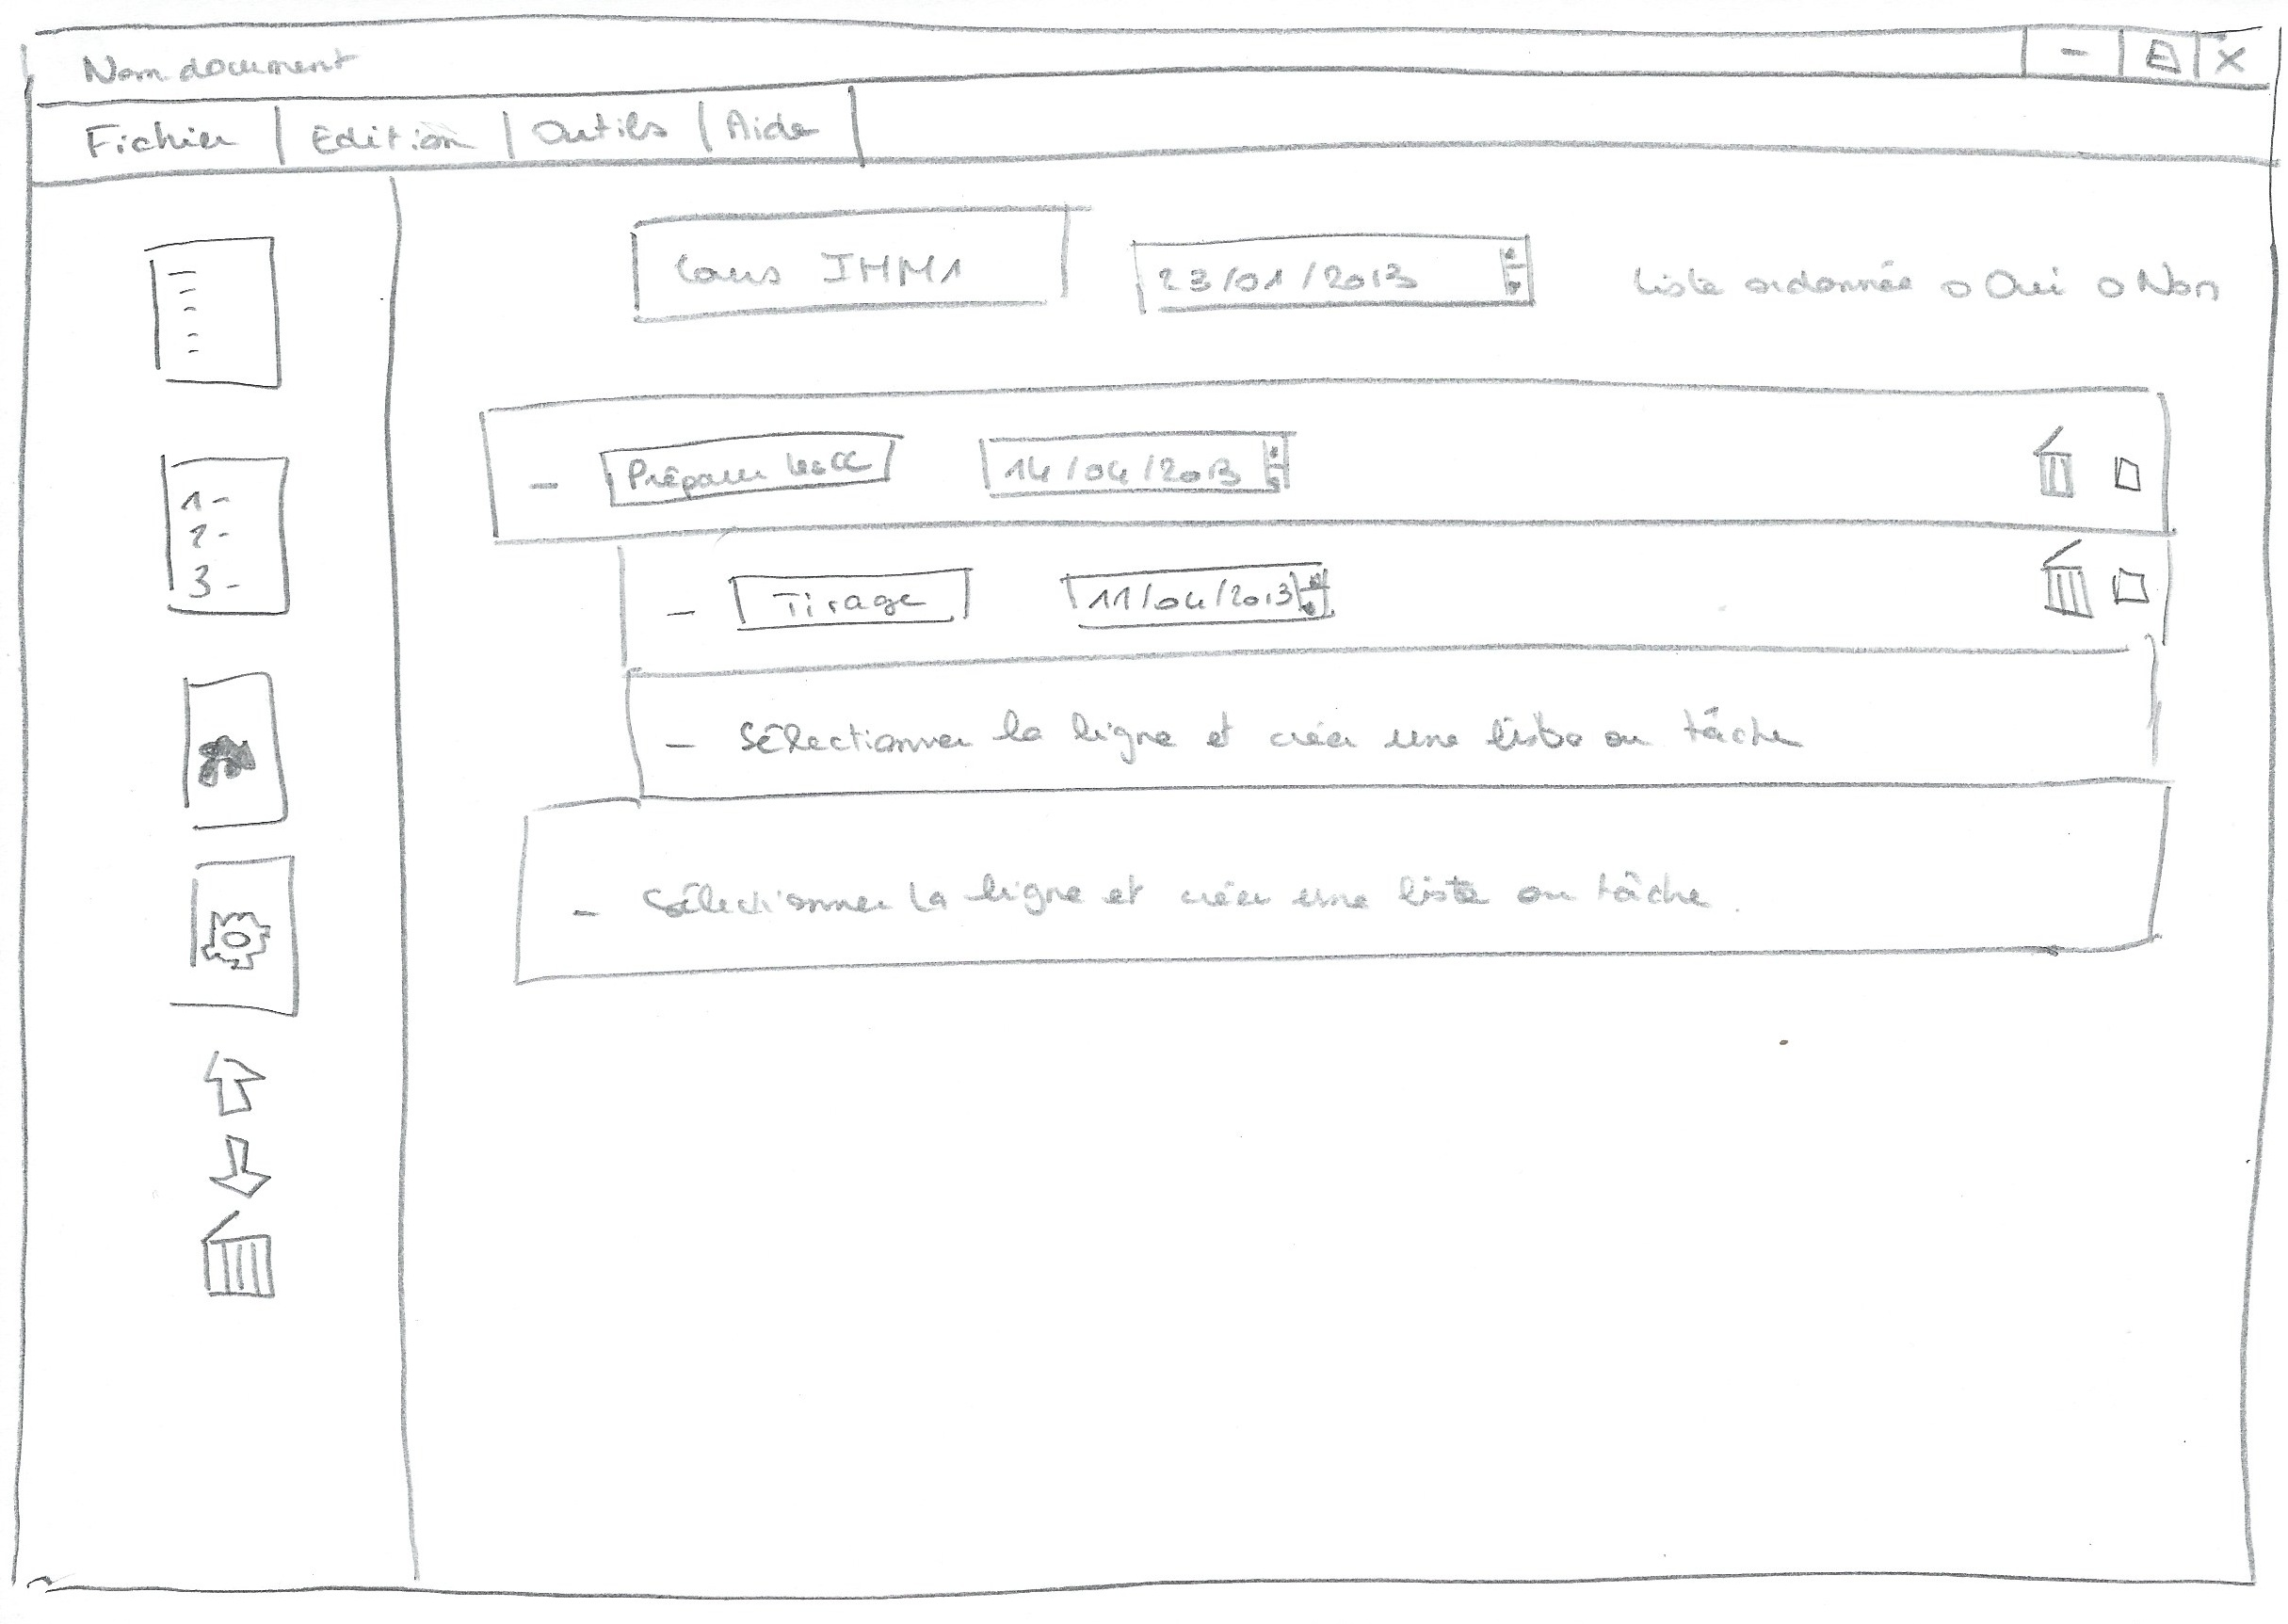
\includegraphics[width=6.8cm]{Images/maquette8.jpeg}
    \caption{\paperPrototyping}
\end{figure}

\subsubsection{Choix réalisés}
Dans cette section, nous expliquons les choix effectués, mis en avant dans le \paperPrototyping{} et pourquoi nous avons choisi de mettre en place ces solutions
:
% Nous avons dû faire quelques choix pour la conception de l'interface. Nous vous les présentons ici et surtout nous expliquons pourquoi nous avons choisi telle
% solution:

\begin{itemize}
\item \textbf{Fonctionnalité de création (liste ordonnée ou non et tâche):} nous avons décidé d'adopter un système de sélection de l'élément "fils". Expliquons
ce système. Lorsque l'utilisateur créé une liste, un élément vide de cette liste apparaît. L'utilisateur doit alors sélectionner cet élément et définir de quel
type l'élément sera. Lorsque cet élément à un type, un nouvel élément vide apparaît; l'utilisateur peut alors définir un autre élément et ainsi de suite. Si
l'utilisateur ne souhaite pas continuer à remplir cette liste, il ne tient plus compte des éléments vides.
\item \textbf{Fonctionnalité \textit{Monter} et \textit{Descendre}:} nous avons décidé de placer ces fonctionnalités dans la boîte à outils plutôt que sur
l'élément à déplacer pour un gain de temps au niveau de l'utilisation. En effet, si nous avions fait le choix de mettre les boutons \textit{monter} et
\textit{descendre} sur l'élément, lorsque l'utilisateur aurait déplacé l'élément, il aurait perdu le focus de la souris sur ces boutons.
Attention, lors de l'utilisation de cette fonctionnalité dans une liste ordonnée; si on monte ou descend un élément de tel façon qu'un élément coché se trouve
être en dessous d'un élément non coché dans la liste, alors le déplacement ne sera pas activé. (Cette dernière précaution n'a pas été implémentée)
\item \textbf{Fonctionnalité \textit{Supprimer}:} nous avons choisi d'ajouter cette possibilité de suppression sur chaque élément pour que l'utilisateur puisse
supprimer plus rapidement. De  plus nous avons décidé de faire apparaître une fenêtre d'avertissement car la suppression d'une liste sélectionnée peut entraîner
la suppression d'éléments. Pour plus de sécurité, le focus de la validation de la suppression est par défaut sur \textit{Non}.
\item \textbf{Fonctionnalité \textit{Paramètre}:} nous avons décidé pour cette fonctionnalité (qui peut entraîner la suppression de différents éléments) de
faire, également, apparaître une fenêtre d'avertissement. Dans cette fenêtre le focus de la validation du changement est mise à \textit{Non}. On perd
cependant un peu de vitesse d'exécution (si l'utilisateur souhaite effectivement bien effectuer ce changement) au profit de plus de sécurité.
% \item \textbf{Widget désactivé :} nous avons décidé de griser tout menu, bouton inutilisable à un état de l'application afin que l'utilisateur n'exécute pas
% d'actions impossibles. Cela évitera qu'il se pose des questions s'il voit aucun changement effectué.
\end{itemize}

\subsection{Scénarios}
Afin de tester notre paper Prototype, nous avons créé plusieurs scénarios.
\subsubsection{Scénario 1 - Création/Utilisation/Suppression de liste}
Ce premier scénario a été utilisé pour tester le \paperPrototyping. Il permet de créer une liste non ordonnée et d'y ajouter une liste ordonnée avec ses propres
tâches et des tâches.
\begin{enumerate}
\item{L'utilisateur choisit quel type de liste il souhaite créer, il choisit ici une liste non ordonnée. Il lui donne un nom et une date de fin. (Pour notre scénario cette liste sera appelée la liste mère)}
\item{Il crée ensuite une liste ordonnée (qui est le premier élément de la liste mère). Il lui donne un nom et une date. (Pour notre scénario cette liste sera appelée la liste 1)}
\item{Il crée ensuite une tâche qui sera le premier élément de la liste 1. Il lui donne un nom et une date. (Pour notre scénario cette tâche sera appelée la tâche 1.1)}
\item{Il créer ensuite une tâche qui sera le deuxième élément de la liste 1. Il lui donne un nom et une date. (Pour notre scénario cette tâche sera appelée la tâche 1.2)}
\item{Il souhaite maintenant échanger les tâches 1.1 et 1.2, il sélectionne donc la tâche 1.1 et la place au dessous de la tâche 1.2}
\item{Une popup peut apparaître et informe l'utilisateur que l'action qu'il vient d'effectuer provoque un conflit de date. Le champs date concerné par le conflit prend une couleur orange d'avertissement.}
\item{L'utilisateur change le type de la liste 1 en une liste non ordonnée.}
\item{L'utilisateur supprime la tâche 1.2}
\item{L'utilisateur supprime la tâche 1. Une popup apparaît pour l'avertir que cette suppression supprimera aussi tous les éléments de la liste.}
\end{enumerate}

\subsubsection{Scénario 2 - Utilisation des templates}
Ce scénario permet de créer une liste à partir d'un template. De modifier cette liste et de la réenregistrer comme un nouveau template.
\begin{enumerate}
\item{L'utilisateur choisit de créer une liste à partir d'un template. Il choisit ici le template qui correspond à la préparation d'un cours, puis donne un nom et une date à sa liste.}
\item{Il va ensuite pour tous les éléments de ce template donner une date.}
\item{L'utilisateur va ensuite modifier cette liste en y ajoutant une tâche à la liste mère (il lui donne un nom et une date).}
\item{Il va ensuite vouloir enregistrer cette nouvelle liste comme un nouveau template.}
\end{enumerate}


%%%%%%%%%%%%%%%%%%%%%%%%%%%%%%%%%%%%%%%%%%%%%%%%%%%%%%%%%%%%%%%%%%%%%%%%%%%%%
%%%%%%%%%%  Etape 3
%%%%%%%%%%%%%%%%%%%%%%%%%%%%%%%%%%%%%%%%%%%%%%%%%%%%%%%%%%%%%%%%%%%%%%%%%%%%%
\newpage
\section{L'IHM}

% \item \textbf{Widget désactivé :} nous avons décidé de griser tout menu, bouton inutilisable à un état de l'application afin que l'utilisateur n'exécute pas
% d'actions impossibles. Cela évitera qu'il se pose des questions s'il voit aucun changement effectué.

Afin de créer une interface la plus simple et explicite possible pour l'utilisateur nous avons effectué différents choix que nous allons expliquer ci-dessous.

La fenêtre principale est tout d'abord composée d'un menu, d'une boite à outils et d'une zone réservée à l'affichage de la liste en cours de création.
\begin{figure}[H]
    \center
    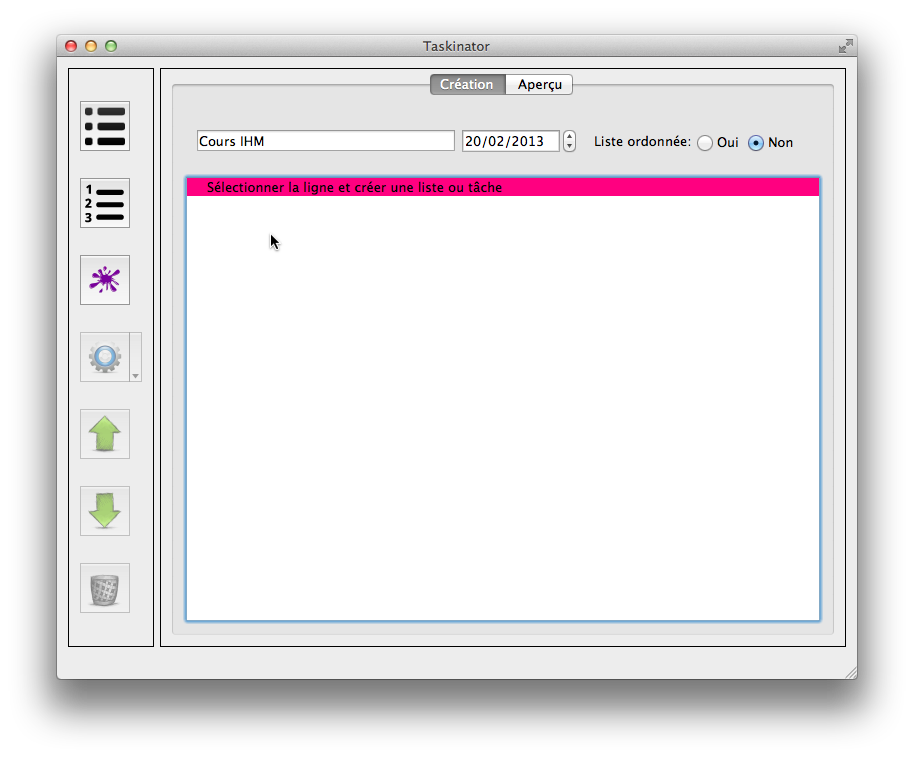
\includegraphics[width=14cm]{Images/mainWindow.png}
    \caption{La fenêtre principale}
\end{figure}

\subsection{Le menu}
Le menu permet de regrouper différentes fonctionnalités sous un thème/rubrique.
On retrouvera les fonctionnalités suivantes:
\begin{itemize}
%%%%%%%%%%%%%%%%%%%%%%% Fichier %%%%%%%%%%%%%%%%%%%%%%%
\item Fichier
\begin{itemize}
\item \textbf{Nouveau:} qui permet de créer une nouvelle liste vide ou à partir d'un template.
\item \textbf{Ouvrir:} qui permet d'ouvrir une liste au format \textit{.tor} enregistrer sur le disque dur de l'utilisateur.
\item \textbf{Ouvrir récent:} qui permet à l'utilisateur d'ouvrir l'une des cinq dernières listes ouvertes dans cette application.
\item \textbf{Enregistrer:} qui permet à l'utilisateur d'enregistrer sa liste en cours à chemin déjà spécifié.
\item \textbf{Enregistrer sous :} qui permet à l'utilisateur de choisir le chemin auquel il souhaite enregistrer sa liste et de l'enregistrer.
\item \textbf{Exporter:} qui permet à l'utilisateur d'exporter sa liste au format PDF. (Cette fonctionnalitée n'a pas été implémentée)
\item \textbf{Quitter:} qui permet à l'utilisateur de quitter l'application.
\end{itemize}
\begin{figure}[H]
    \center
    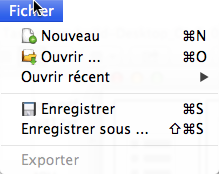
\includegraphics[width=2cm]{Images/menuFichier.png}
    \caption{Le menu Fichier}
\end{figure}
%%%%%%%%%%%%%%%%%%%%%%% Edition %%%%%%%%%%%%%%%%%%%%%%%
\item Édition
\begin{itemize}
\item \textbf{Annuler:} qui permet à l'utilisateur d'annuler une action qu'il vient d'effectuer. (Cette fonctionnalitée n'a pas été implémentée)
\item \textbf{Rétablir:} qui permet à l'utilisateur de rétablir une action qu'il vient d'annuler. (Cette fonctionnalitée n'a pas été implémentée)
\end{itemize}	
\begin{figure}[H]
    \center
    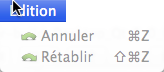
\includegraphics[width=2cm]{Images/menuEdition.png}
    \caption{Le menu Fichier}
\end{figure}
%%%%%%%%%%%%%%%%%%%%%%% Outils %%%%%%%%%%%%%%%%%%%%%%%
\item Outils
\begin{itemize}
\item \textbf{Enregistrer template:} qui permet à l'utilisateur d'enregistrer sa liste en tant que template au format \textit{.ulk}.
\item \textbf{Option:} qui permet à l'utilisateur de gérer ses templates. Il peut choisir le chemin vers lequel il souhaite enregistrer ses templates. La liste des templates présents est affichée. On peut sélectionner un template et afficher sa structure. On peut de plus importer ou supprimer un template .
\end{itemize}
\begin{figure}[H]
    \center
    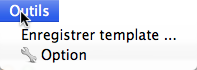
\includegraphics[width=2cm]{Images/menuOutils.png}
    \caption{Le menu Fichier}
\end{figure}
%%%%%%%%%%%%%%%%%%%%%%% Aide %%%%%%%%%%%%%%%%%%%%%%%
\item Aide
\begin{itemize}
\item \textbf{A propos:} permet à l'utilisateur d'avoir plus d'information sur l'application \textit{Taskinator}.
\end{itemize}
\end{itemize}

\subsection{Boite à outils}
Cette boite à outils permet de rassembler toutes les fonctionnalités que l'utilisateur sera amené à utiliser fréquemment. Nous avons décidé de mettre cette boite à outils à gauche, puisque dans notre culture le sens de lecture est de gauche à droite. Toutes les fonctionnalités présentent dans cette boîte à outils seront appliquées sur l'élément sélectionné dans la zone d'affichage de la liste. Cette boite à outils contient les fonctionnalités suivantes:
\begin{itemize}
\item \textbf{Créer une liste non ordonnée (
\includegraphics[width=0.25cm]{Images/list.png}) :} elle permet à l'utilisateur de créer une nouvelle liste non ordonnée.
\item \textbf{Créer une liste ordonnée (
\includegraphics[width=0.25cm]{Images/list_ordered.png}) :} elle permet à l'utilisateur de créer une nouvelle liste ordonnée.
\item \textbf{Créer une tâche (
\includegraphics[width=0.25cm]{Images/task.png}) :} elle permet à l'utilisateur de créer une nouvelle tâche.
\item \textbf{Paramètre (
\includegraphics[width=0.25cm]{Images/gnome-system.png}) :} elle permet à l'utilisateur de changer le type d'un élément.
\item \textbf{Monter (
\includegraphics[width=0.25cm]{Images/arrow_up.png}) :} elle permet à l'utilisateur de monter un élément.
\item \textbf{Descendre  (
\includegraphics[width=0.25cm]{Images/arrow_down.png}) :} elle permet à l'utilisateur de descendre un élément.
\item \textbf{Supprimer  (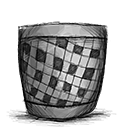
\includegraphics[width=0.25cm]{Images/trash_empty.png}) :}  elle permet à l'utilisateur de supprimer un élément.
\end{itemize}
Tous les boutons permettant de réaliser ces fonctionnalités ont été implémentés grâce à des \textit{QToolButton}. Nous avons ensuite utilisé des signaux et des slots afin de connecter l'action à réaliser aux boutons.

\subsection{Zone d'affichage de la liste}
Cette zone est comme indiqué réservée à l'affichage de la liste en cours de création. On pourra donc voir l'arborescence de la liste, avec toutes ses informations.
Cette zone sera organisée en une arborescence d'éléments. Pour cela, nous avons utilisé un \textit{QTreeWidget}. Celui-ci sera composé d'éléments.

Nous avons créé notre propre élément (héritant de \textit{QWidget}) composé d'un \textit{QLineEdit} permettant de taper le nom de l'élément, d'un \textit{QDateEdit} permettant de rentrer la date, d'un \textit{QToolButton} permettant d'ajouter la fonctionnalité de suppression sur l'élément et d'une \textit{QCheckBox} permettant de valider la réalisation de la tâche.
Plusieurs cas sont possible pour l'état de la checkbox:
\begin{itemize}
\item Dans le cas d'un élément d'une liste ordonnée, cette checkbox sera grisée si la tâche antérieure n'est pas cochée.
\item Dans le cas ou l'élément est une liste, tant que la checkbox de la liste est grisée, tous les éléments fils ont des checkbox grisées.
\item Dans le cas d'une liste, sa checkbox sera automatiquement cochée lorsque tous les éléments de la liste seront eux aussi cochés.
\end{itemize}
\begin{figure}[H]
    \center
    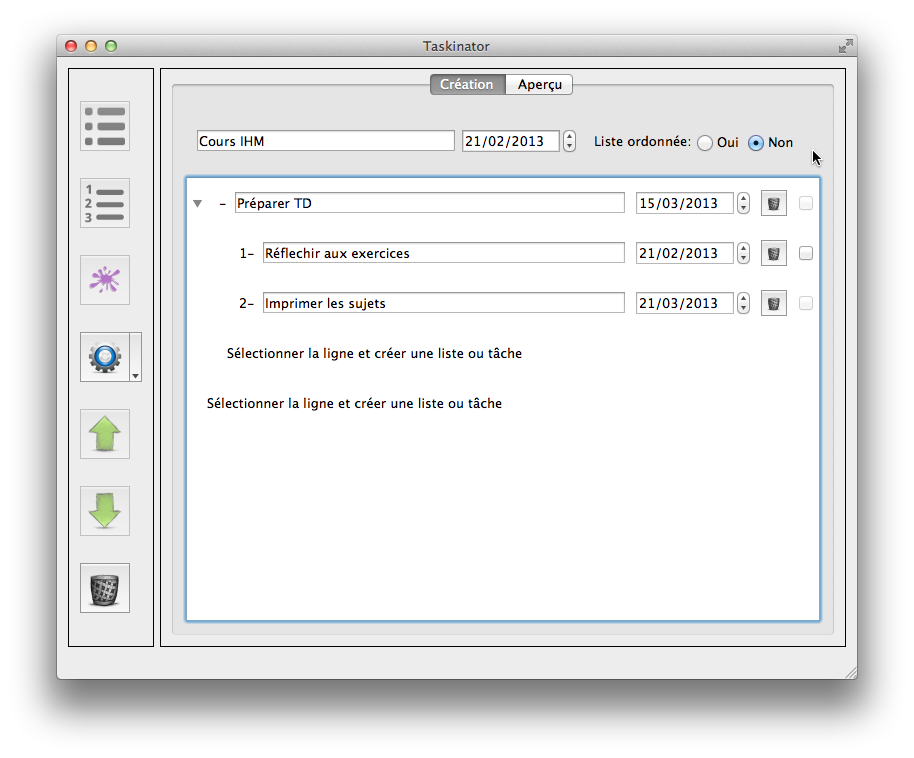
\includegraphics[width=7.4cm]{Images/caseDesactive.png}
    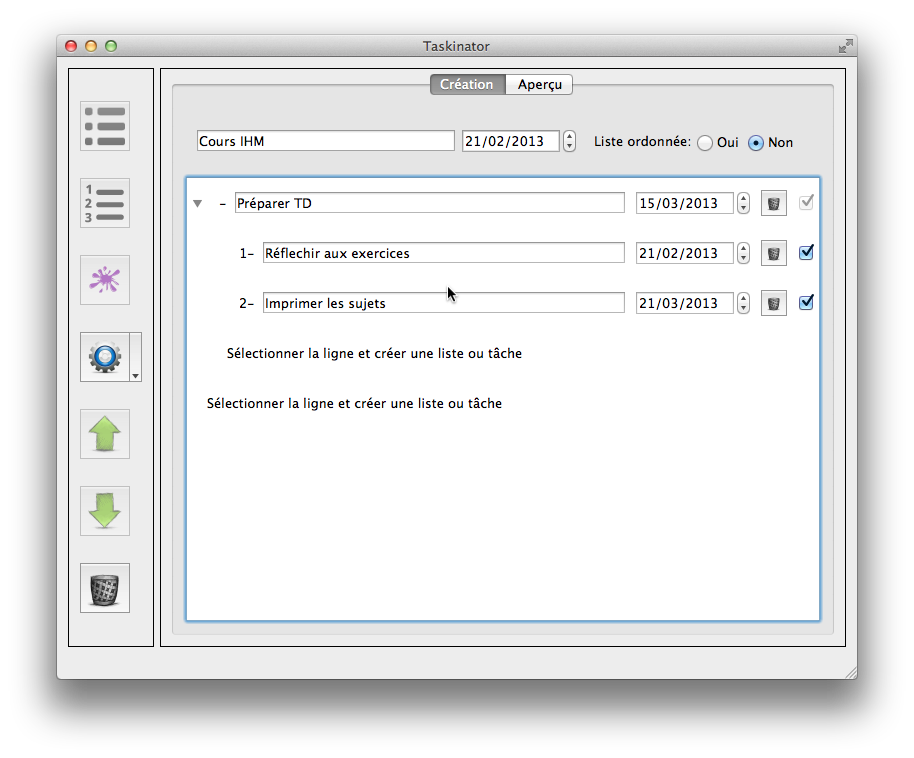
\includegraphics[width=7.4cm]{Images/checkboxListe.png}
    \caption{Fonctionnement de l'activation/désactivation des cases à cocher}
\end{figure}
Nous aurons une information supplémentaire au début de chaque élément. Dans le cas d'une liste non ordonnées, ses éléments sont représentés avec un tiret devant les informations de la liste, tandis que les éléments des listes ordonnées sont représentés à l'aide de numéro.

Nous avons décidé pour plus de sécurité de griser tout menu, bouton inutilisable à un état de l'application afin que l'utilisateur n'exécute pas
d'actions impossibles. Cela évitera qu'il se pose des questions s'il voit aucun changement effectué. De cette façon l'utilisateur sait à
chaque instant que cette fonctionnalité est présente et n'a pas à chercher si une action particulière peut être effectuée ou pas.

%%%%%%%%%%%%%%%%%%%%%%%%%%%%%%%%%%%%%%%%%%%%%%%%%%%%%%%%%%%%%%%%%%%%%%%%%%%%%
%%%%%%%%%%  Etape 4
%%%%%%%%%%%%%%%%%%%%%%%%%%%%%%%%%%%%%%%%%%%%%%%%%%%%%%%%%%%%%%%%%%%%%%%%%%%%%
\newpage
\section{Le modèle}
Afin de réaliser cette application nous nous sommes basés sur le modèle suivant dont voici le diagramme de classes:
\begin{figure}[htpb]
	\center
	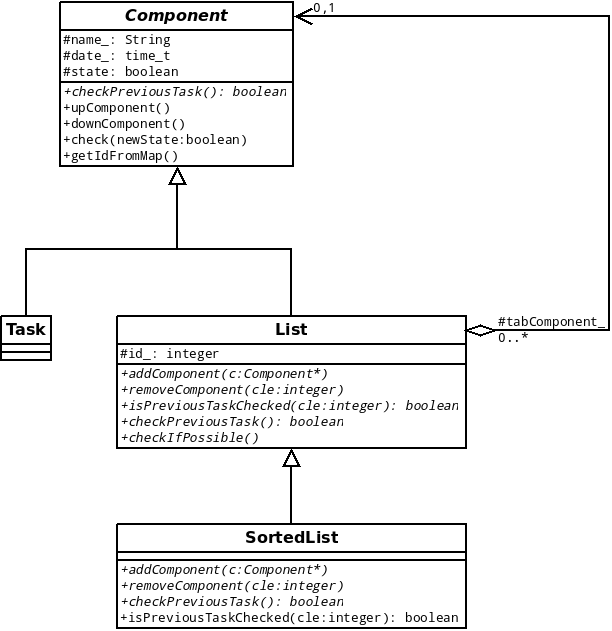
\includegraphics[scale=0.5]{Images/dia_classe.png}
	\caption{Diagramme de classe du modèle}
\end{figure}

Le modèle de cette application est composé d'un pattern composite permettant d'implémenter une structure d'arbre et de composer les différents objets ensemble.
Nous avons donc ici un \textit{Component} qui peut être, soit une \textit{Task} (une tâche), soit une \textit{List} (une liste) qui elle-même peut ensuite être
une \textit{SortedList} (une liste ordonnée), celle-ci hérite de la classe \textit{List}. Ce modèle permet donc comme expliqué ci-dessus de composer ces
éléments et d'obtenir par exemple des listes de listes de tâches \dots 
Nous pouvons donc gérer tous ces composants au sein de ce modèle et ainsi, ajouter un composant dans une liste, le supprimer, le déplacer d'un rang
(dans les deux sens). Nous disposons aussi de toutes les fonctions permettant de déterminer si un composant est cochable ou non.

%%%%%%%%%%%%%%%%%%%%%%%%%%%%%%%%%%%%%%%%%%%%%%%%%%%%%%%%%%%%%%%%%%%%%%%%%%%%%
%%%%%%%%%%  Etape 5
%%%%%%%%%%%%%%%%%%%%%%%%%%%%%%%%%%%%%%%%%%%%%%%%%%%%%%%%%%%%%%%%%%%%%%%%%%%%%
\newpage
\section{Limite de l'application}
%Parler de l'idée du prof, consernant la création de la liste d'une part et le faite de pouvoir cocher d'autre part.
Notre application à ses propres limites. Elle ne permet pas d'éditer différentes listes en même temps (l'utilisateur peut créer/modifier une liste à la fois).

Elle ne gère pas non plus la cohérence des dates des composants. Effectivement dans le cas d'une liste ordonnée, il faudrait vérifier que la date d'une tâche
soit inférieure à la date de la tâche suivante. Cette vérification devra se faire lors de la création mais aussi à chaque action effectuée.

Et ne peut pour le moment pas gérer un historique d'actions effectuées, se qui aurait put être très utile en cas d'erreur de manipulation(à la suite d'une
suppression non souhaitée par exemple).

Il aurait été sympathique de proposer la création de la liste d'une part et de pouvoir cocher les tâches d'autre part, sur deux affichage différents. Que la
modification d'un des deux affichages est un impact sur l'autre.
%TODO A compléter si des idées

%%%%%%%%%%%%%%%%%%%%%%%%%%%%%%%%%%%%%%%%%%%%%%%%%%%%%%%%%%%%%%%%%%%%%%%%%%%%%
%%%%%%%%%%  CONCLUSION GENERALE
%%%%%%%%%%%%%%%%%%%%%%%%%%%%%%%%%%%%%%%%%%%%%%%%%%%%%%%%%%%%%%%%%%%%%%%%%%%%%
\newpage
\section{Conclusion générale}
Ce projet nous a permis de réfléchir à la structure de l'IHM afin que celle-ci soit la plus intuitive possible pour l'utilisateur. Réfléchir à la position des
boutons, le nom ou l'icône les représentant, comment l'ajout des composants se fera au sein de la liste, \ldots{}
Et donc, d'orienter notre conception sur l'IHM, plus que sur le modèle, et ainsi expérimenter une autre approche de conception.
%TODO A compléter

\end{document}